\chapter{Additional Figures}

\begin{figure}[!htbp]
    \centering
    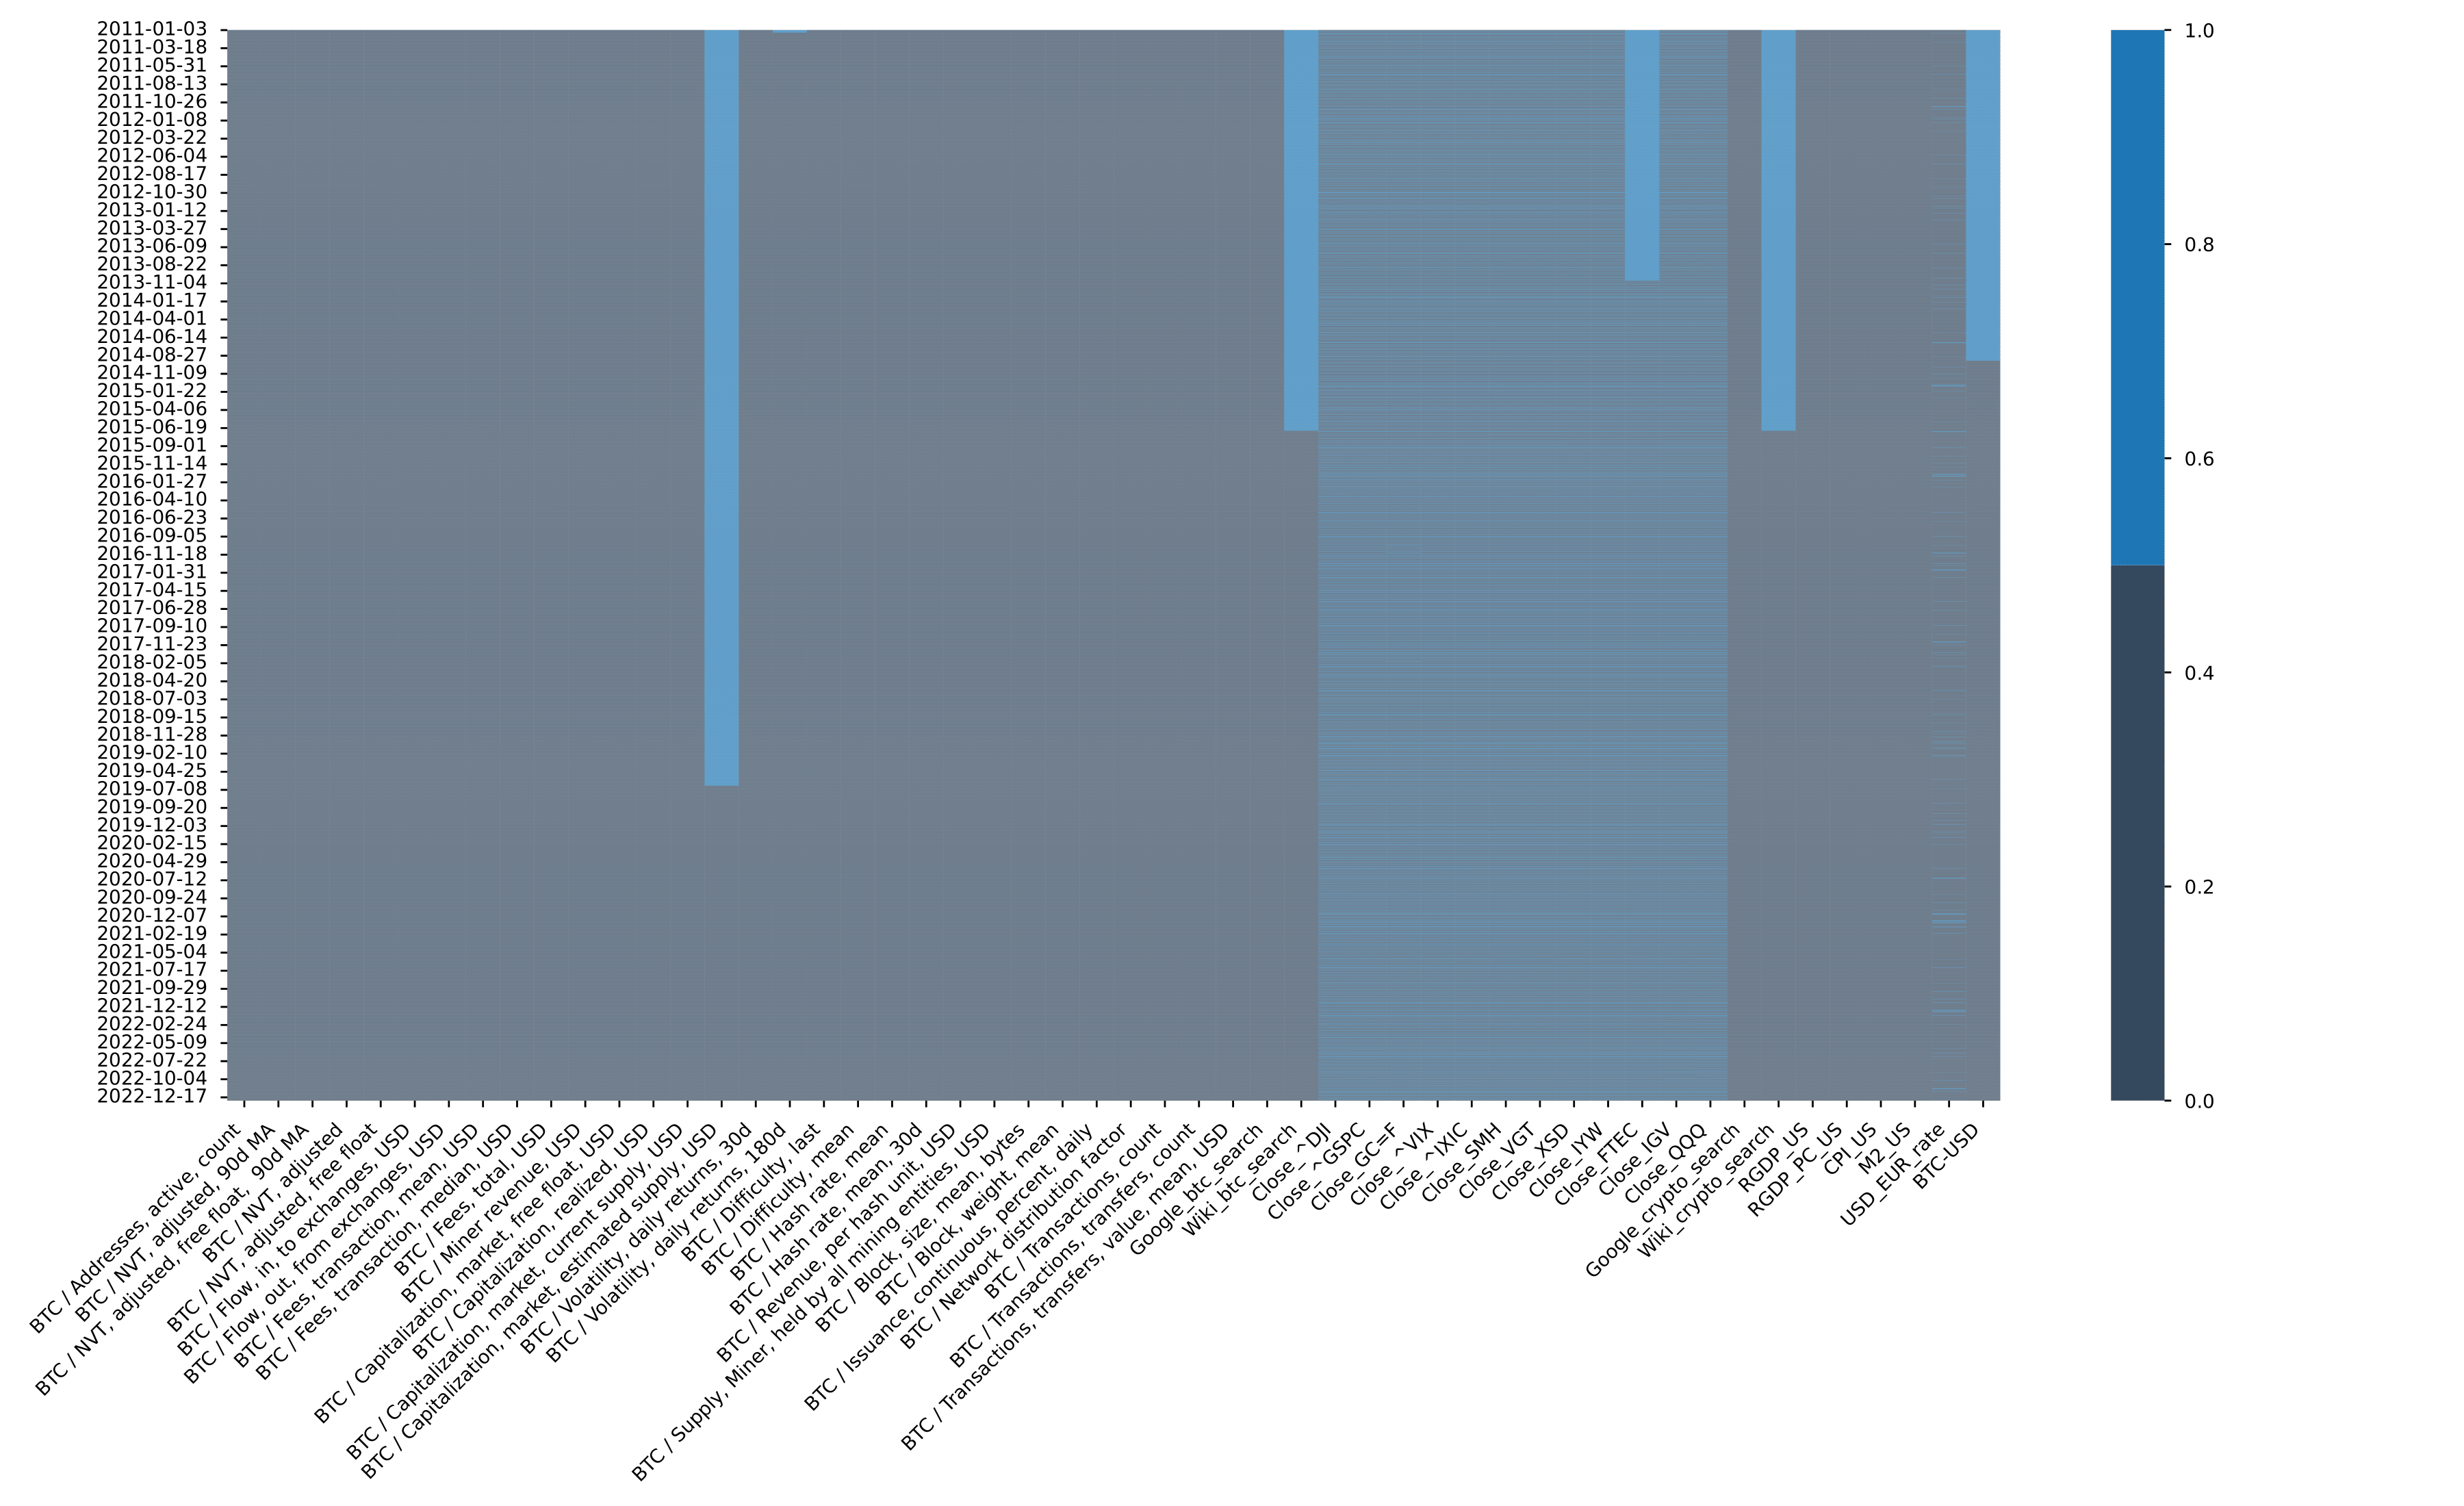
\includegraphics[width=1.1\linewidth,height=0.9\textheight,keepaspectratio]{Figures/BTC_missing_1.png}
    \caption{Missing Values BTC before subsetting}
    \label{fig:btc_missing_1}
    \caption*{Source: Author}
\end{figure}

\begin{figure}[!htbp]
    \centering
    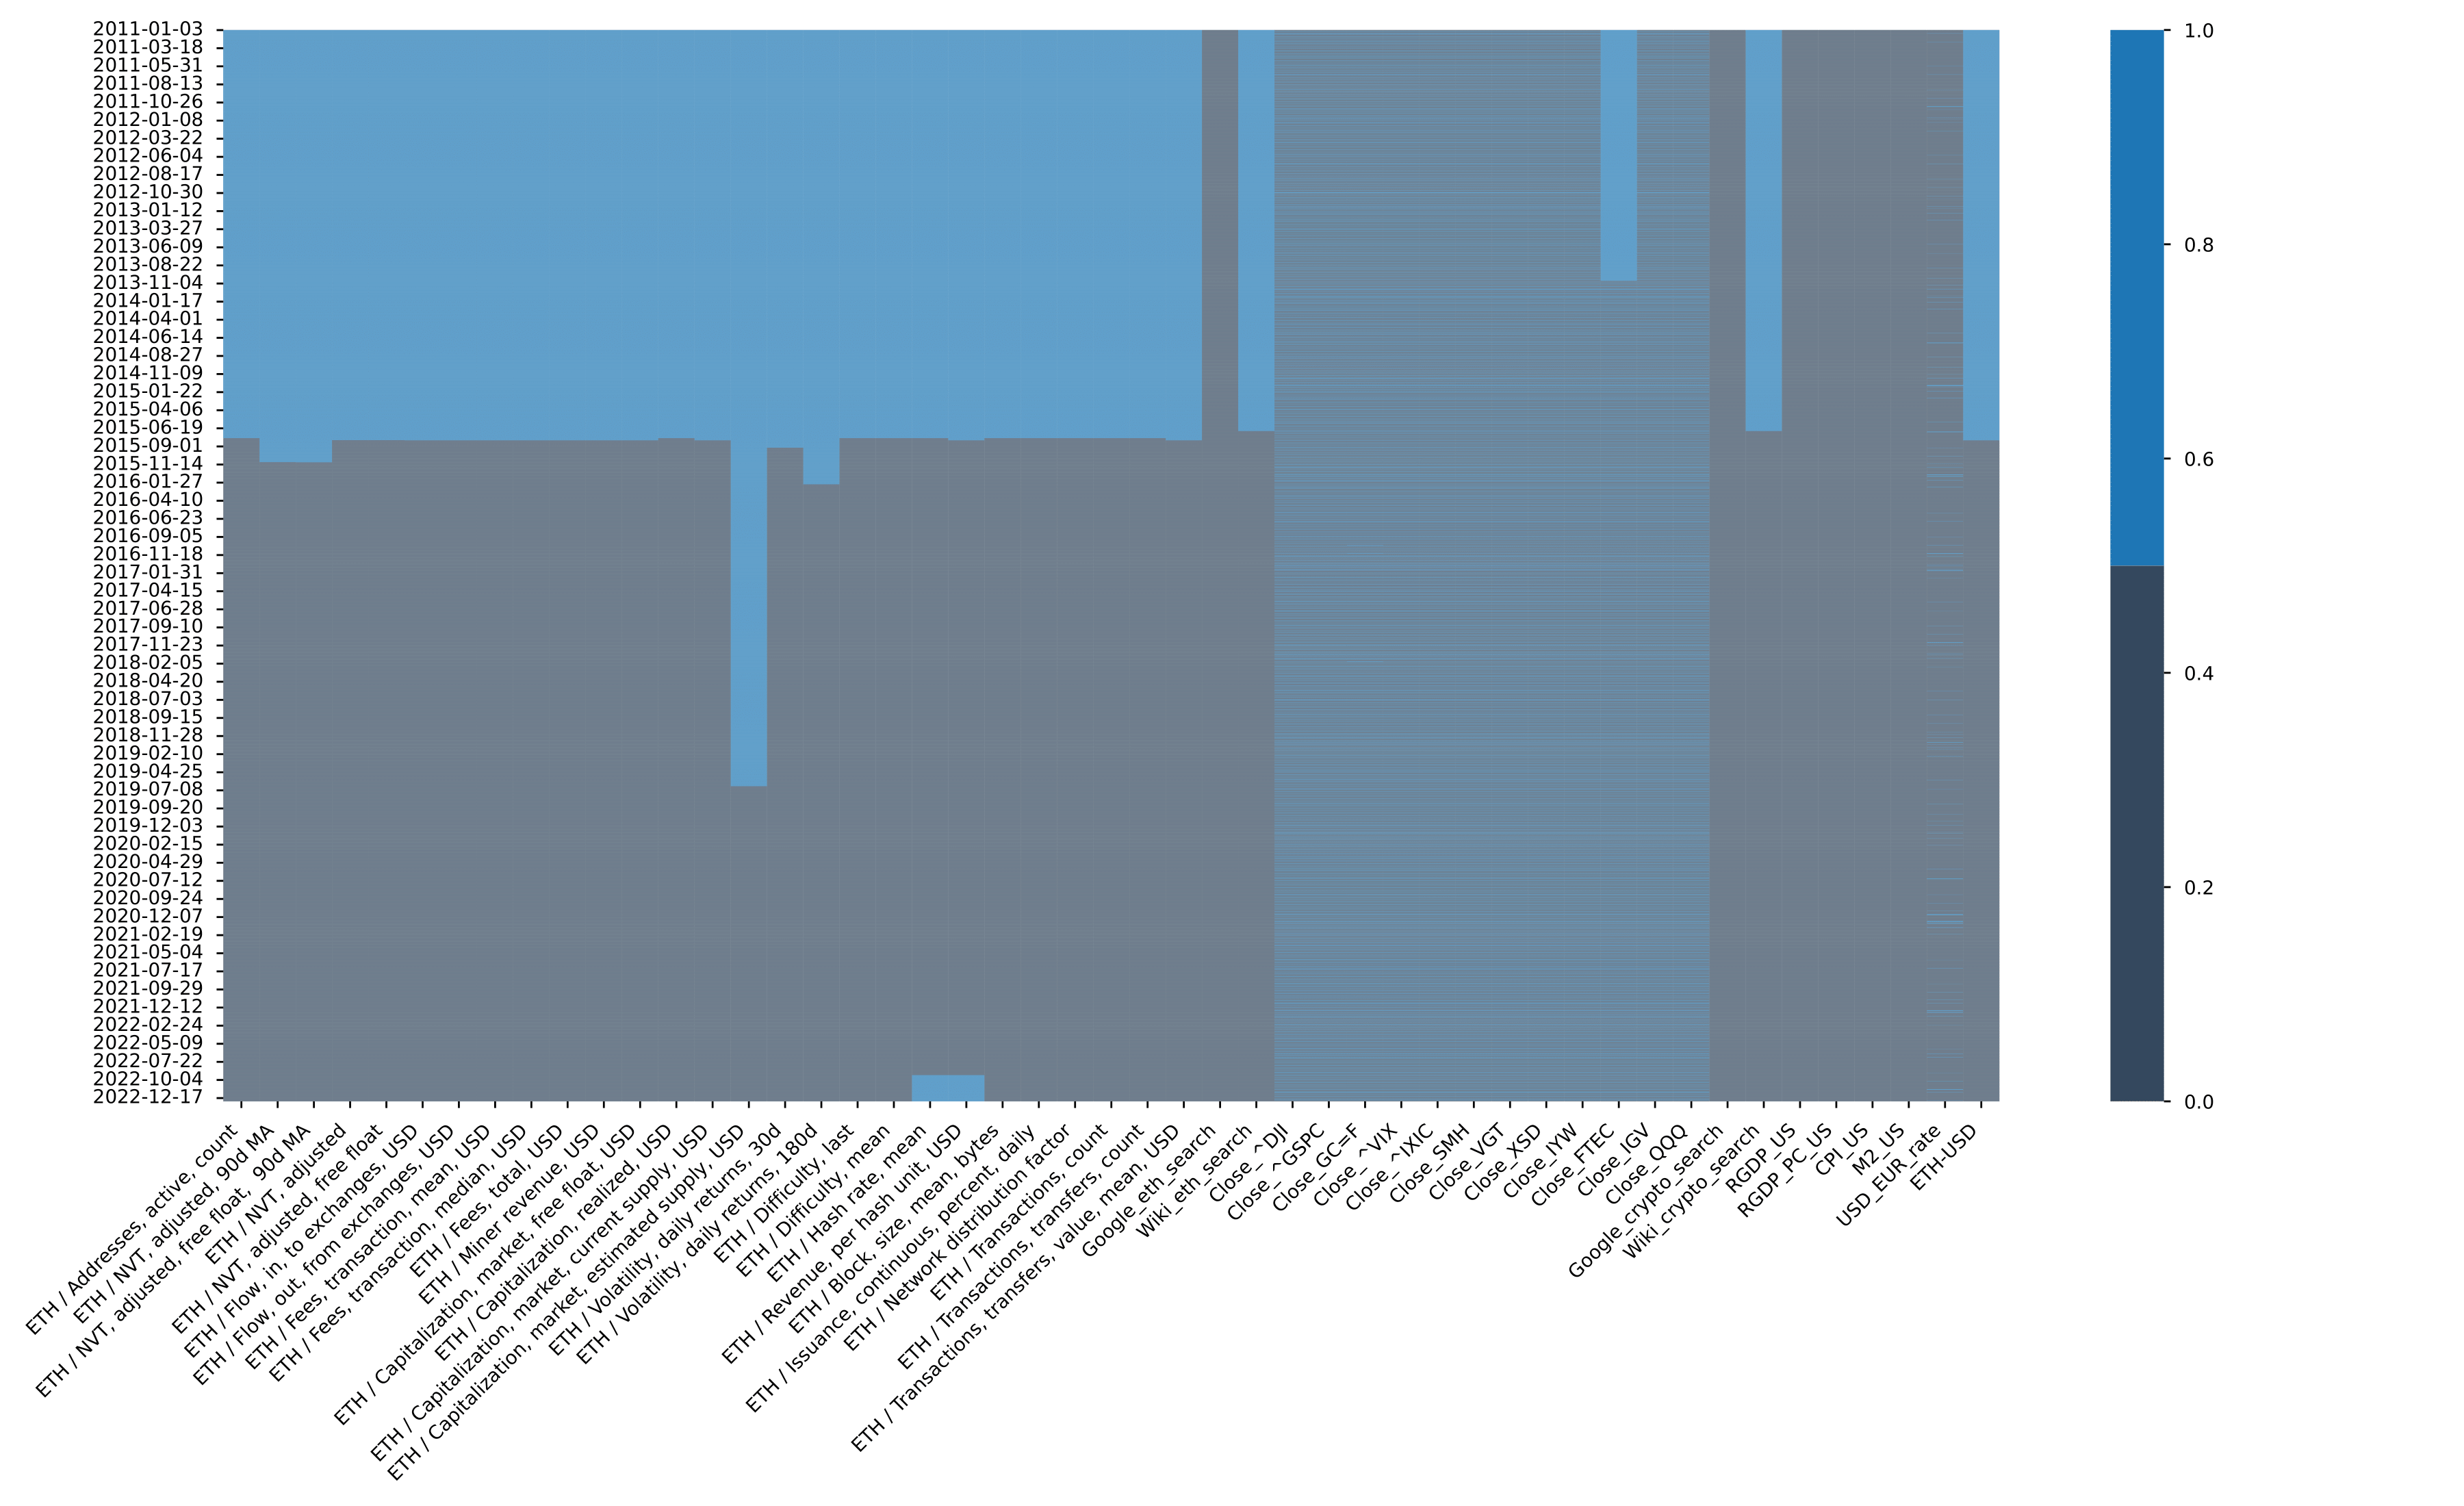
\includegraphics[width=1.1\linewidth,height=0.9\textheight,keepaspectratio]{Figures/ETH_missing_1.png}
    \caption{Missing Values ETH before subsetting}
    \label{fig:eth_missing_1}
    \caption*{Source: Author}
\end{figure}

\begin{figure}[!htbp]
    \centering
    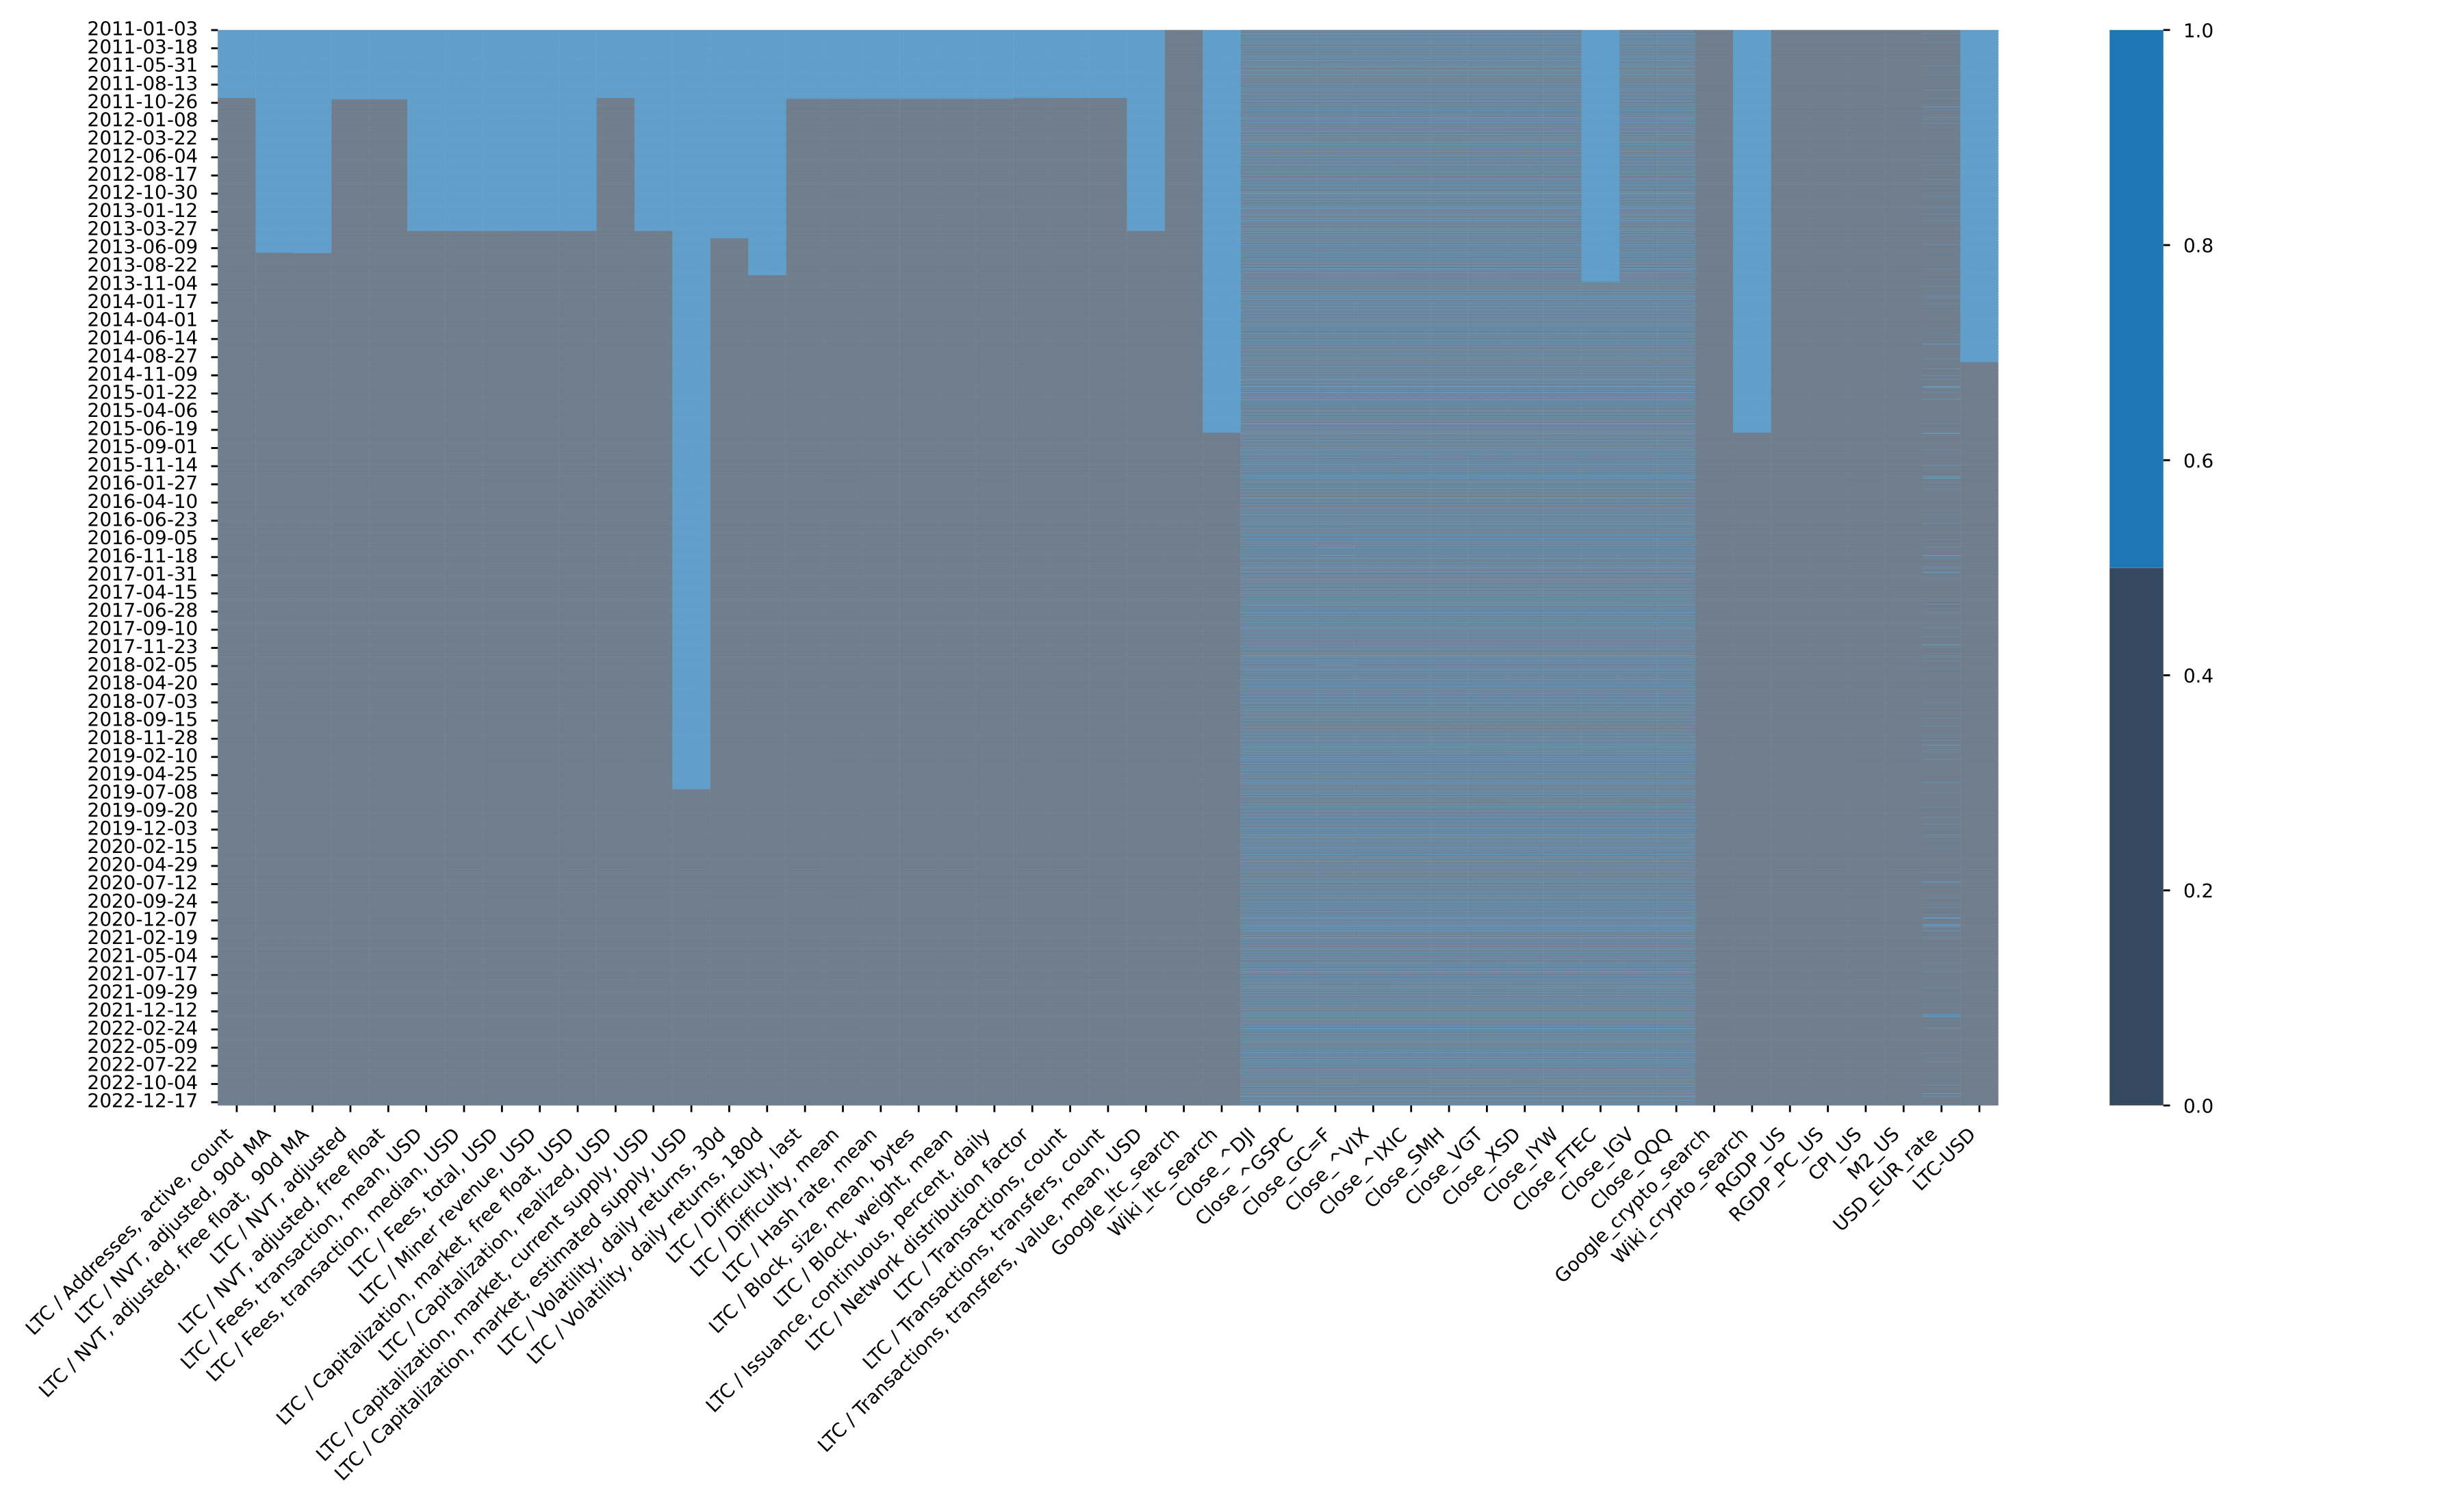
\includegraphics[width=1.1\linewidth,height=0.9\textheight,keepaspectratio]{Figures/LTC_missing_1.png}
    \caption{Missing Values LTC before subsetting}
    \label{fig:ltc_missing_1}
    \caption*{Source: Author}
\end{figure}

\begin{figure}[!h]
    \centering
    \caption{Correlation matrix of the ETH dataset shows high level of 
    multicollinearity.}
    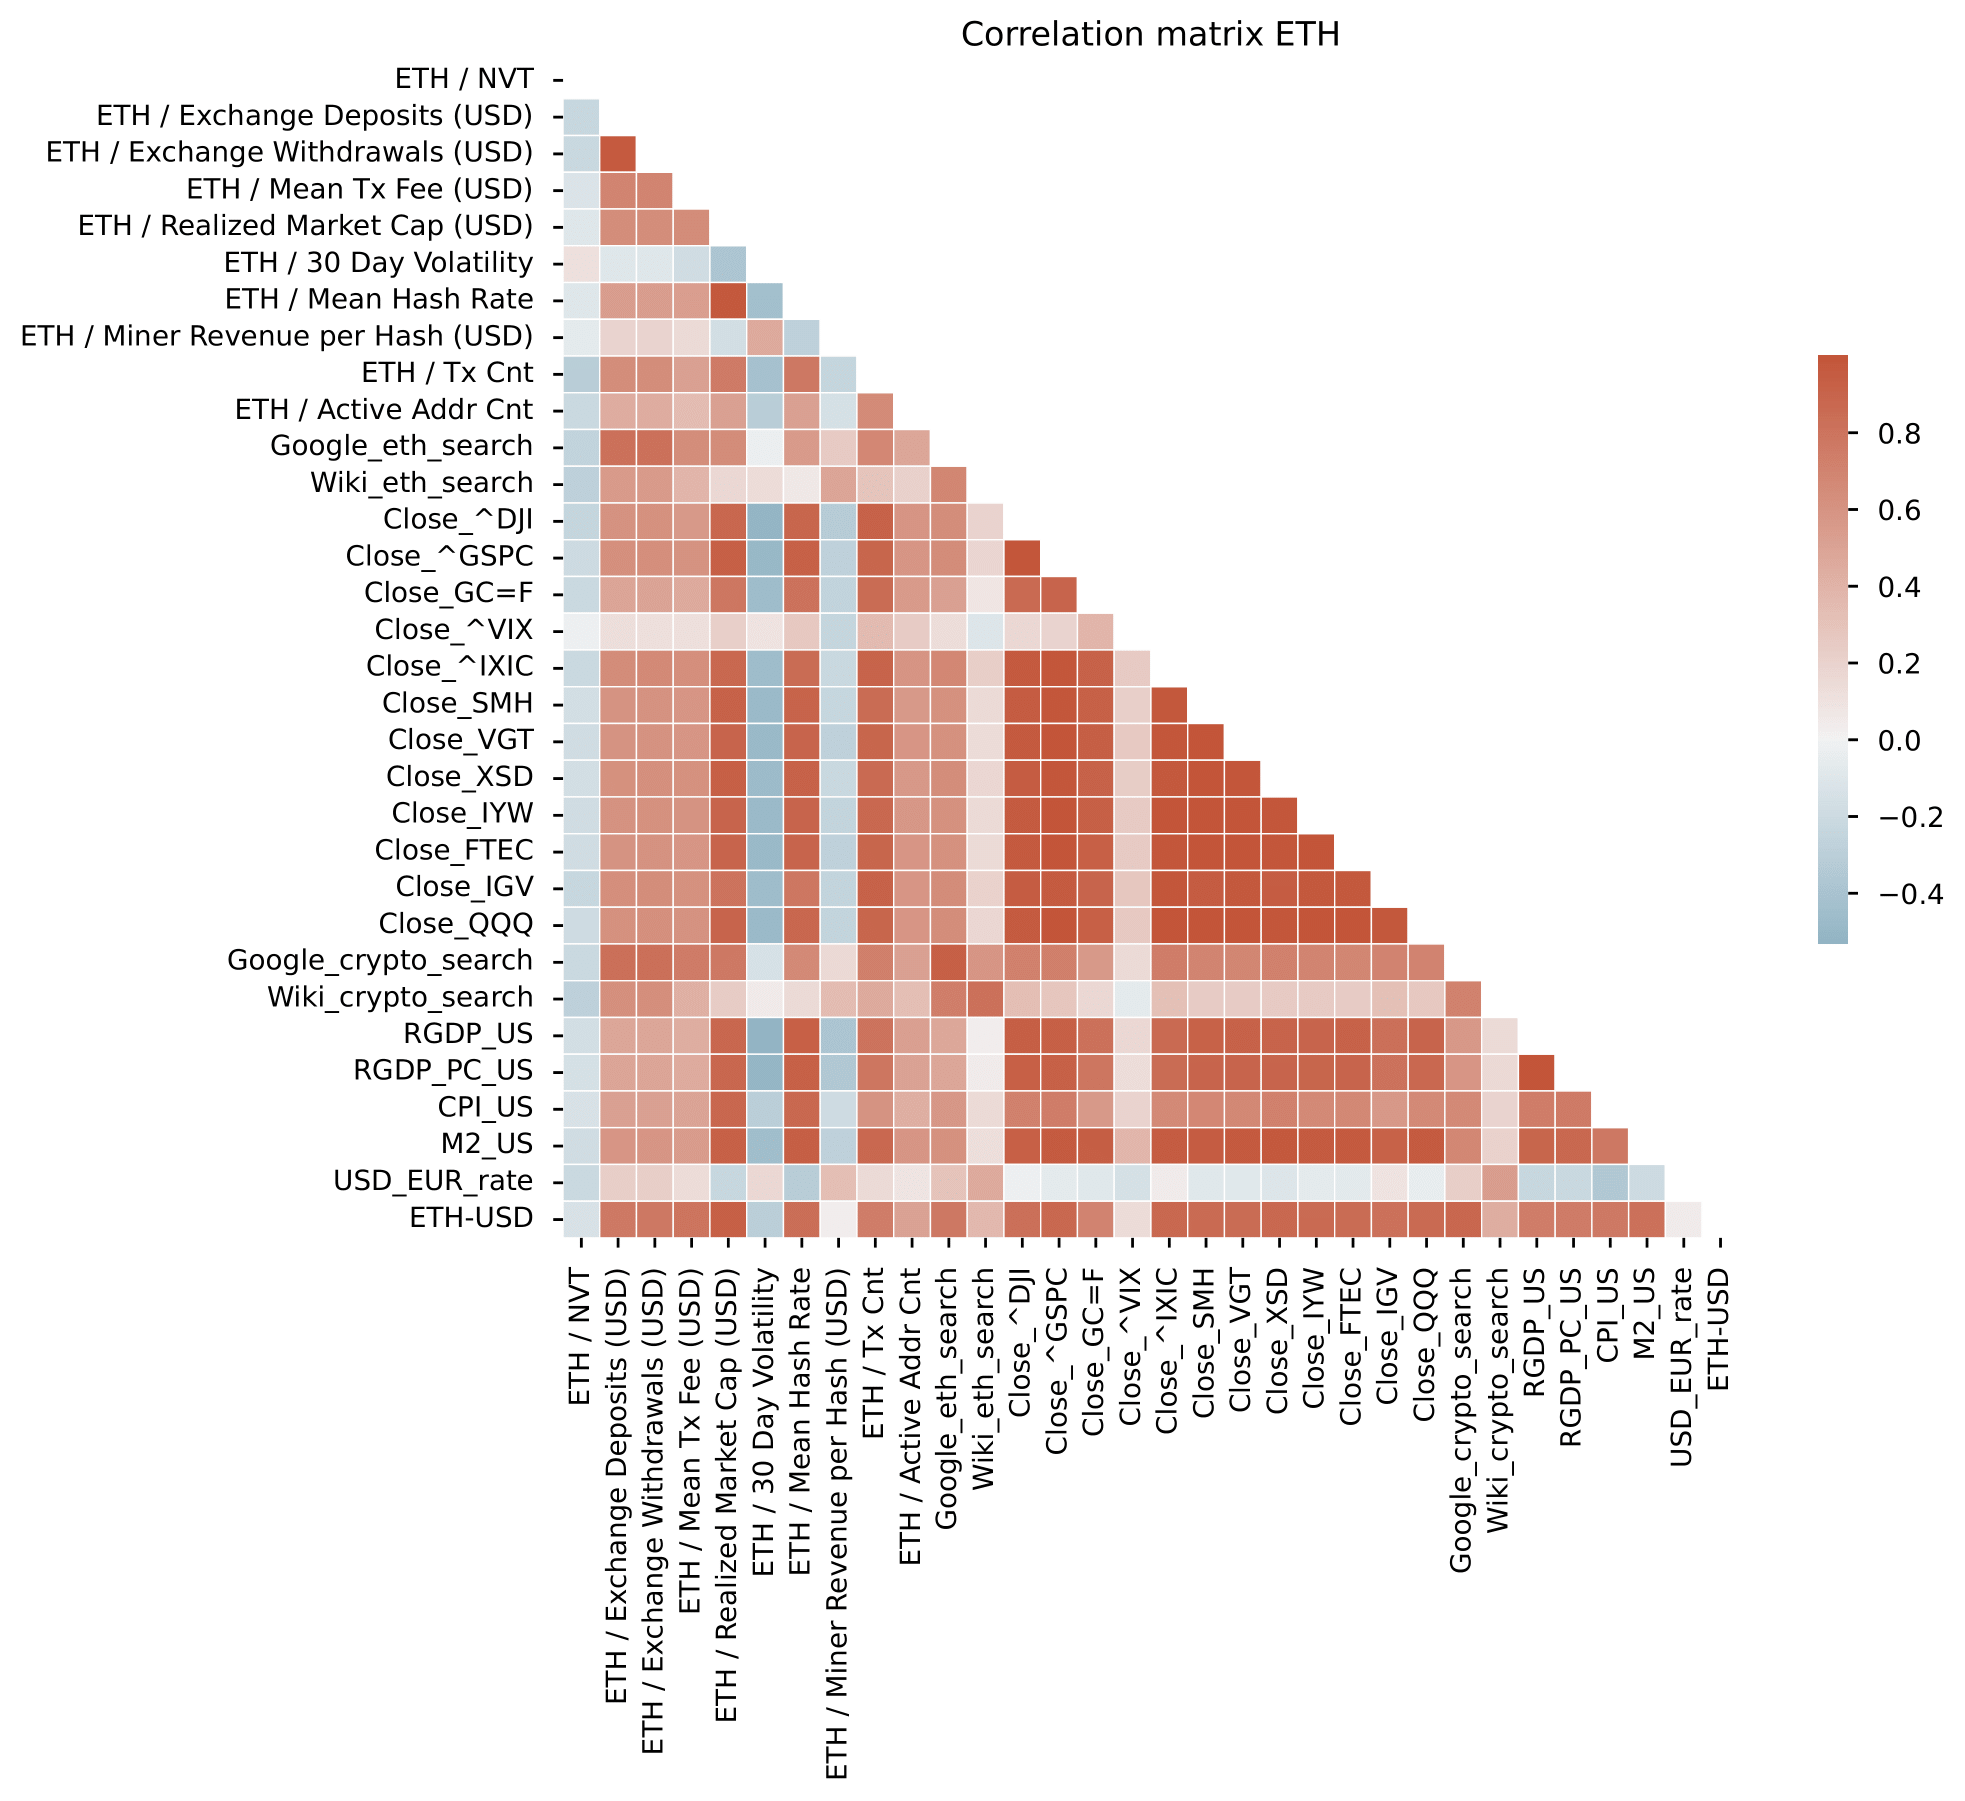
\includegraphics[width=1\textwidth]{Figures/Corr_eth.png}
    \caption*{Source: Author}
    \label{fig:Corr_eth}
\end{figure}

\begin{figure}[!h]
    \centering
    \caption{Correlation matrix of the ETH dataset after
    log differencing all of the variables.}
    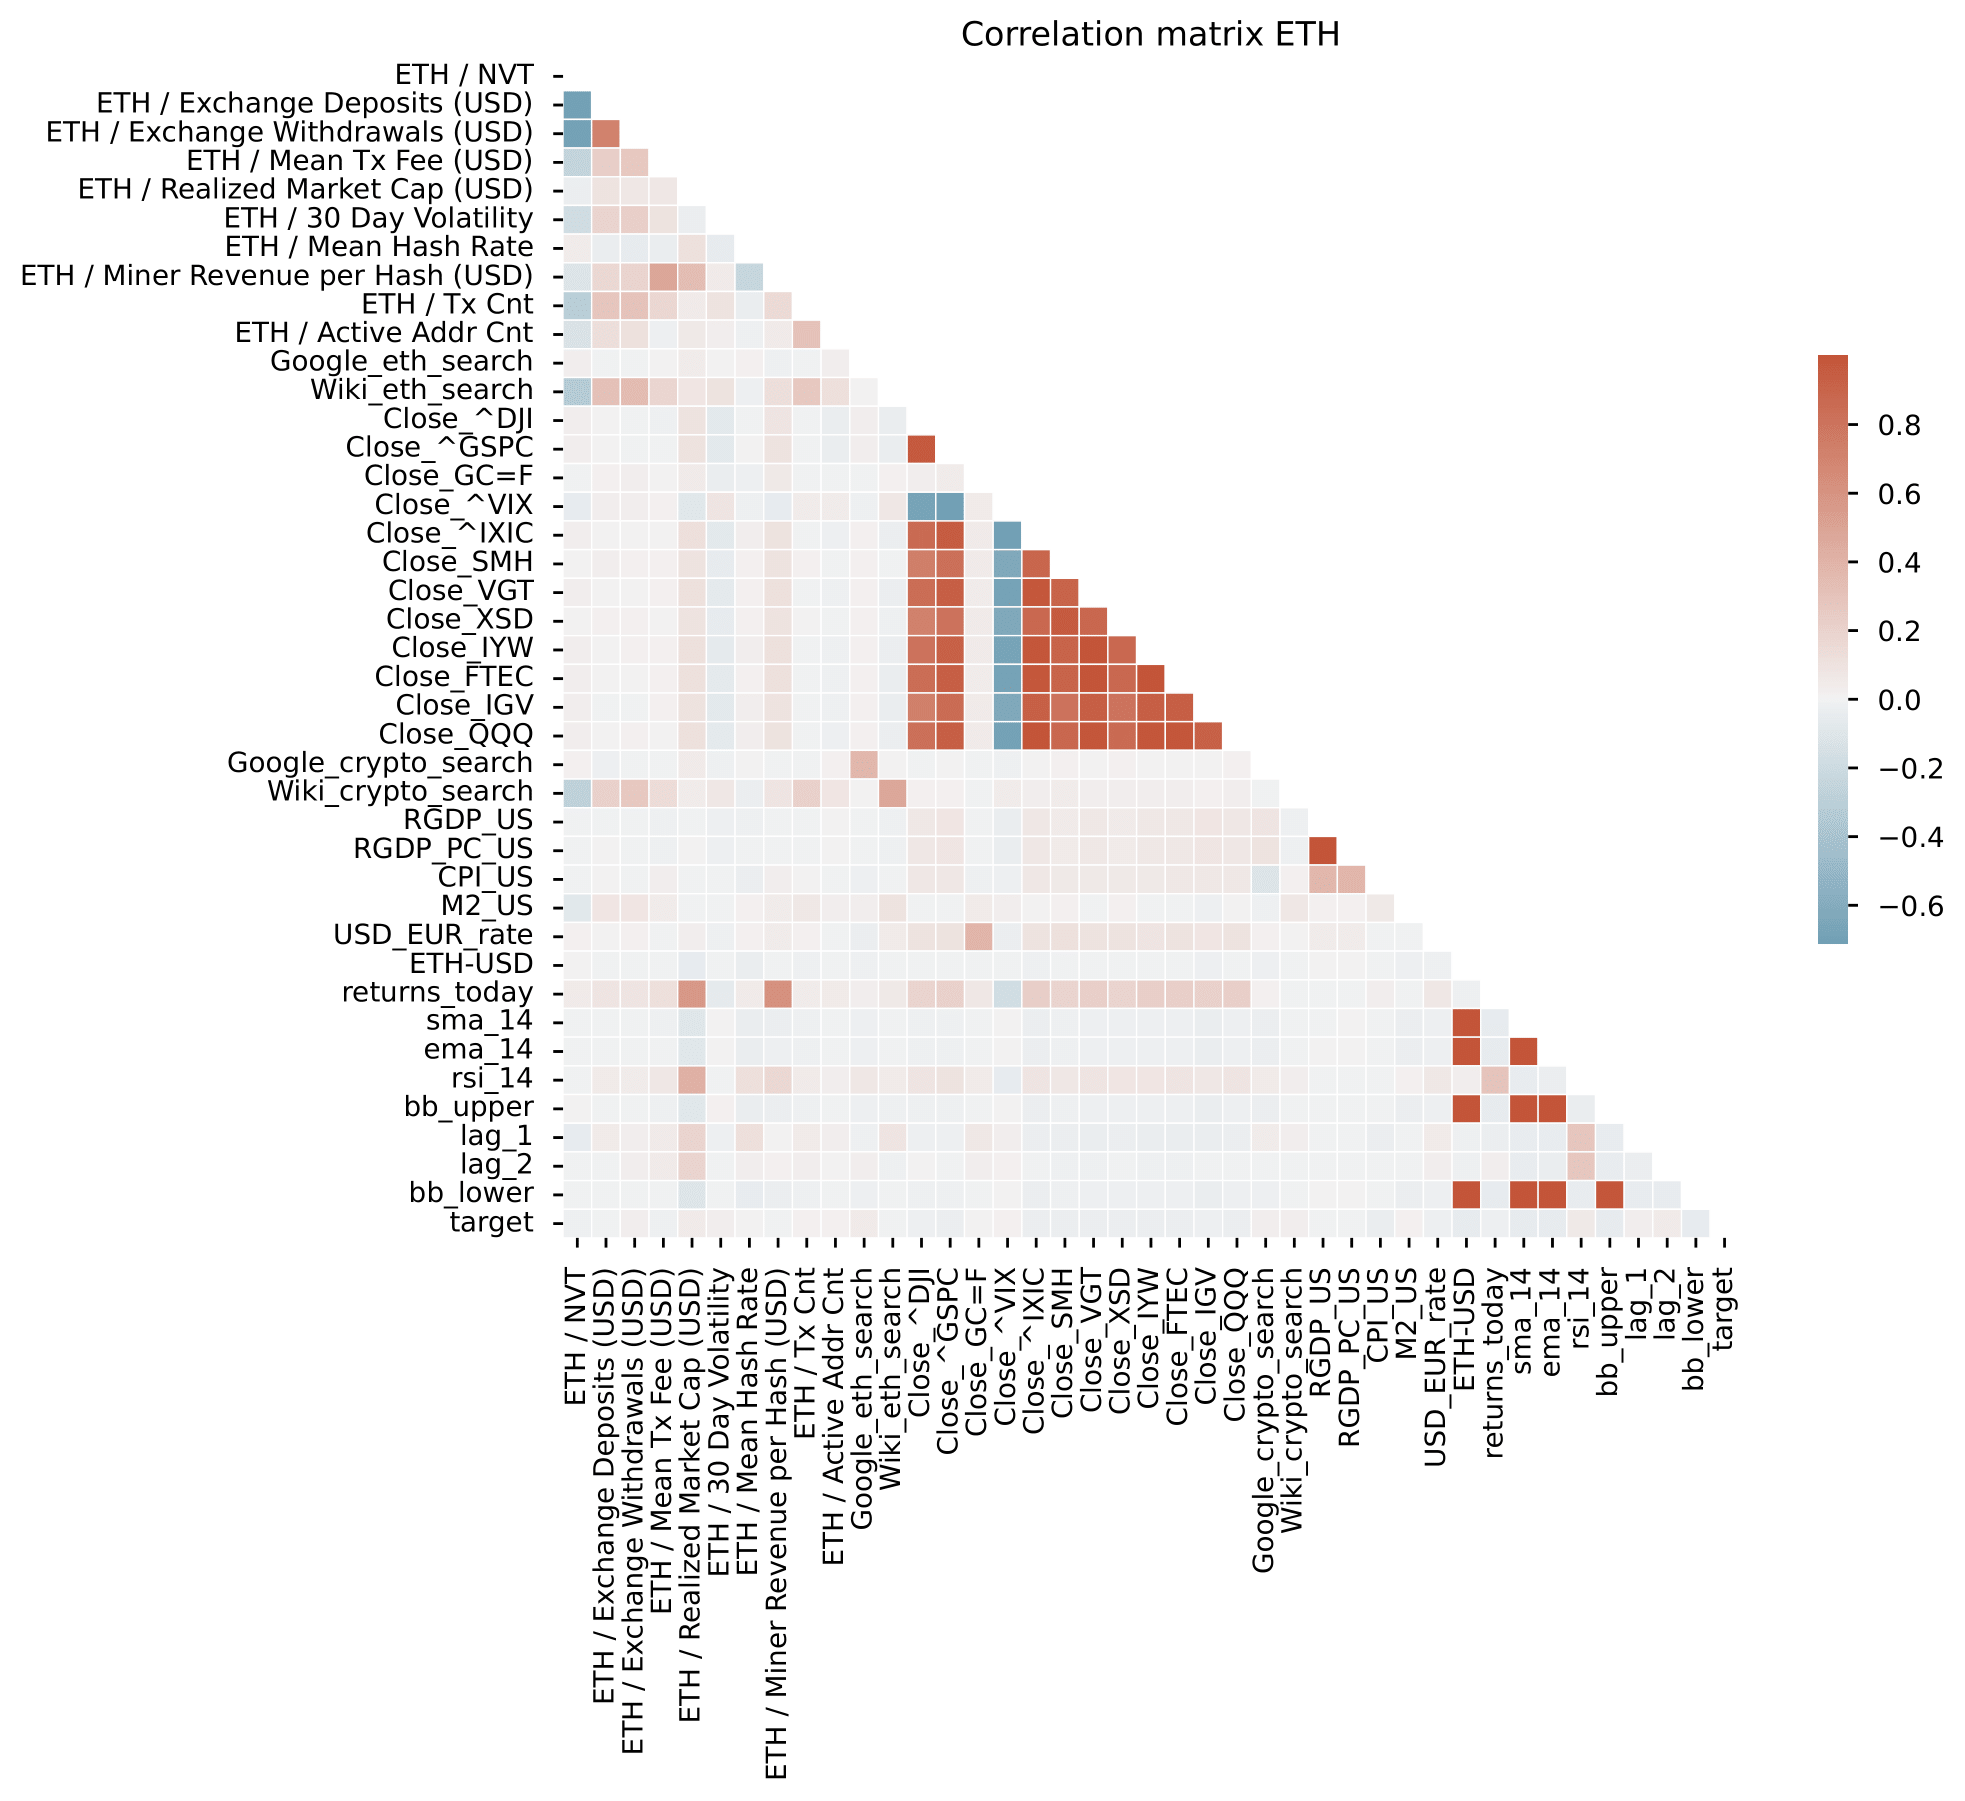
\includegraphics[width=1\textwidth]{Figures/Corr_eth_logdiff.png}
    \caption*{Source: Author}
    \label{fig:Corr_eth_logdiff}
\end{figure}

\begin{figure}[!h]
    \centering
    \caption{Correlation matrix of the LTC dataset shows high level of 
    multicollinearity.}
    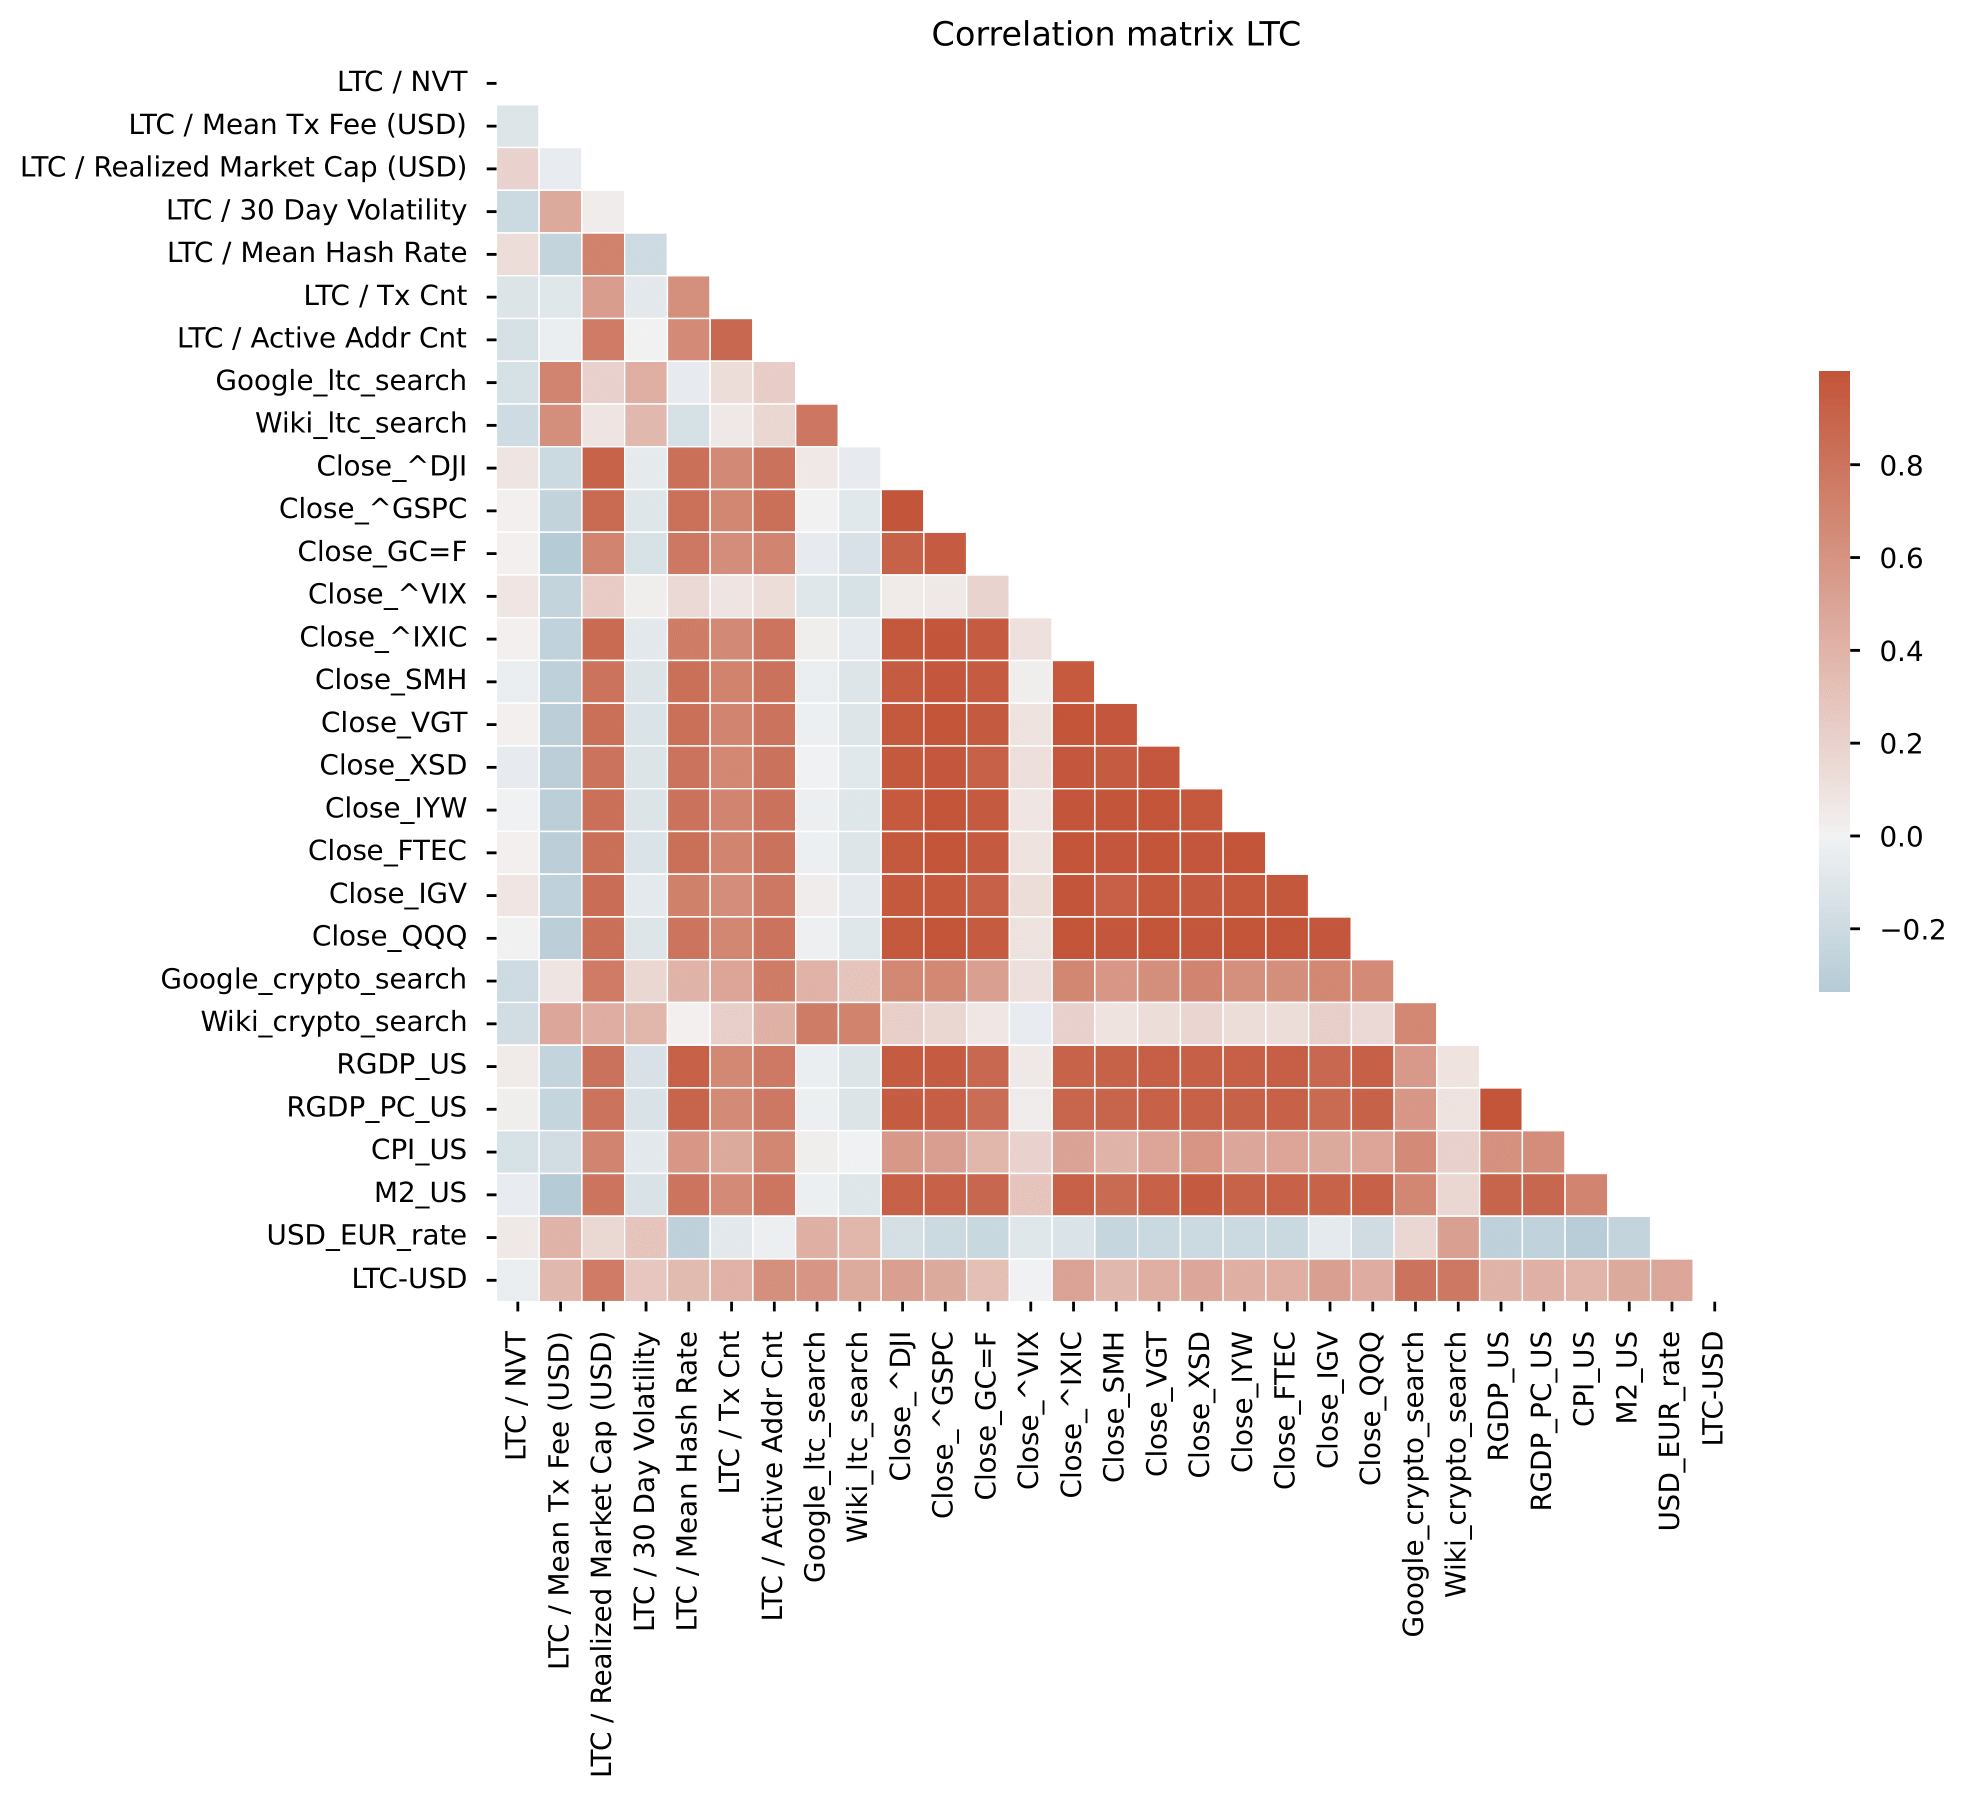
\includegraphics[width=1\textwidth]{Figures/Corr_ltc.png}
    \caption*{Source: Author}
    \label{fig:Corr_ltc}
\end{figure}

\begin{figure}[!h]
    \centering
    \caption{Correlation matrix of the LTC dataset after
    log differencing all of the variables.}
    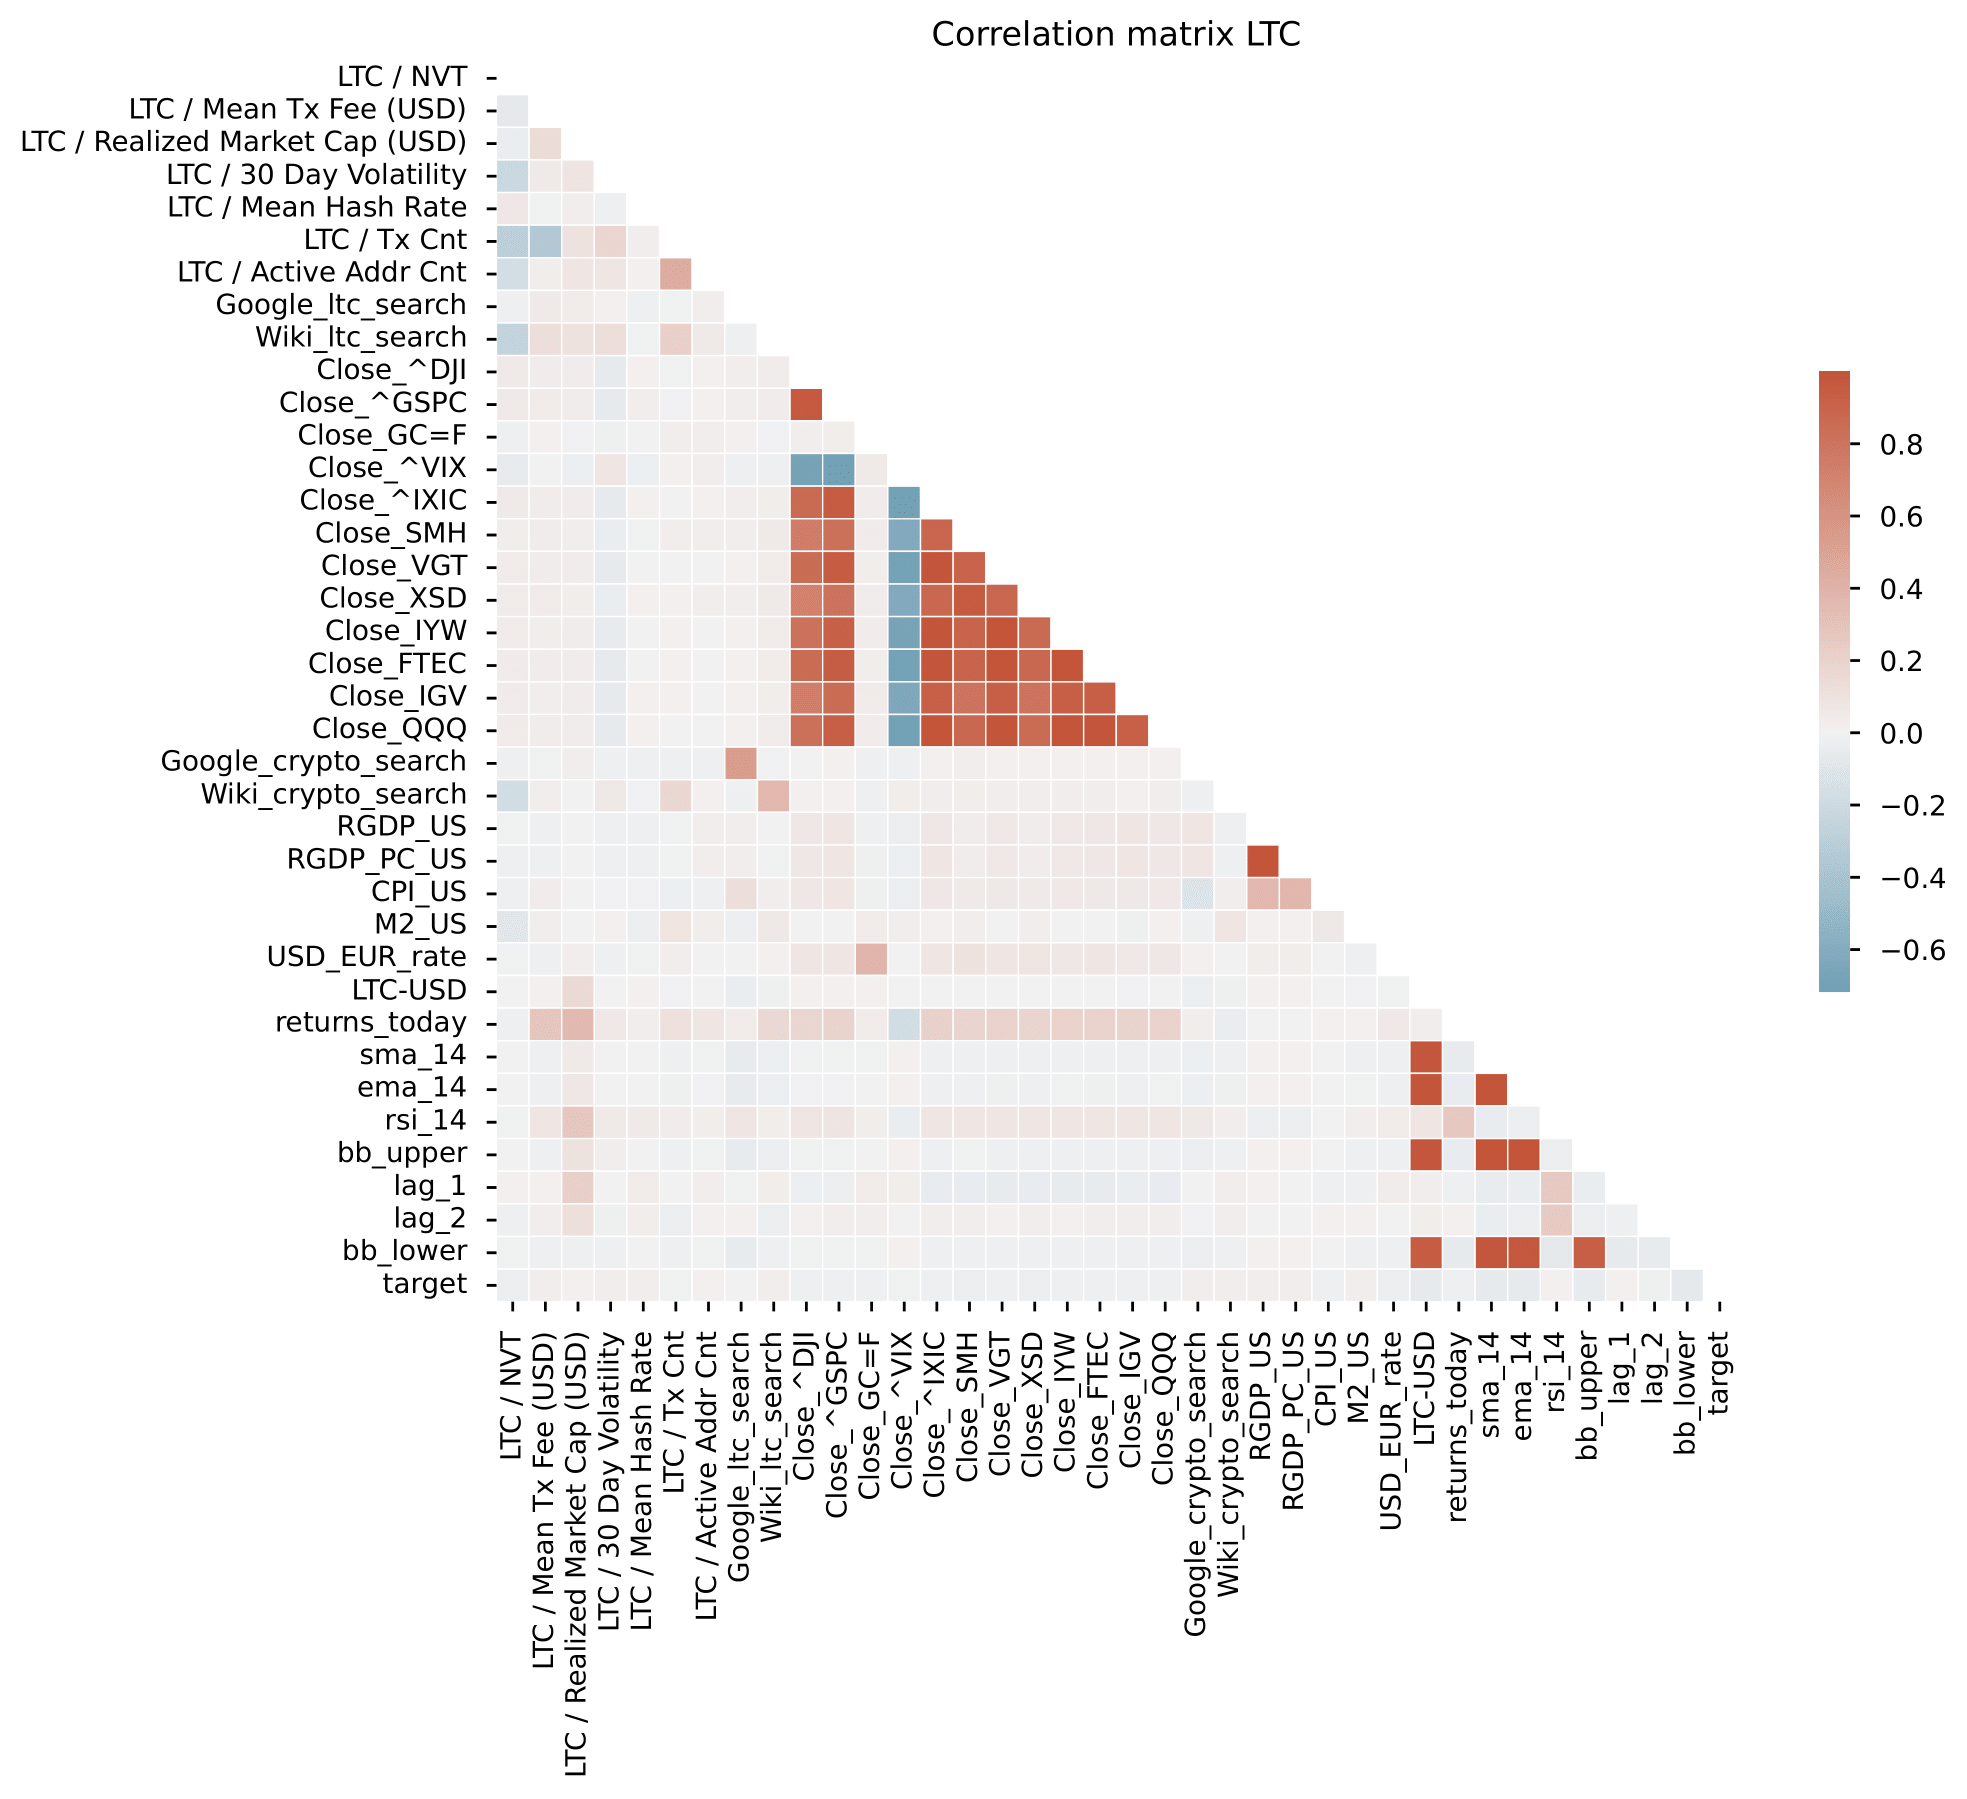
\includegraphics[width=1\textwidth]{Figures/Corr_ltc_logdiff.png}
    \caption*{Source: Author}
    \label{fig:Corr_ltc_logdiff}
\end{figure}


\begin{figure}[!h]
    \centering
    \caption{Learned coefficients of the Ridge regression model
    with incremental training on the ETH dataset. Five 
    coefficients with highest variance are highlighted.}
    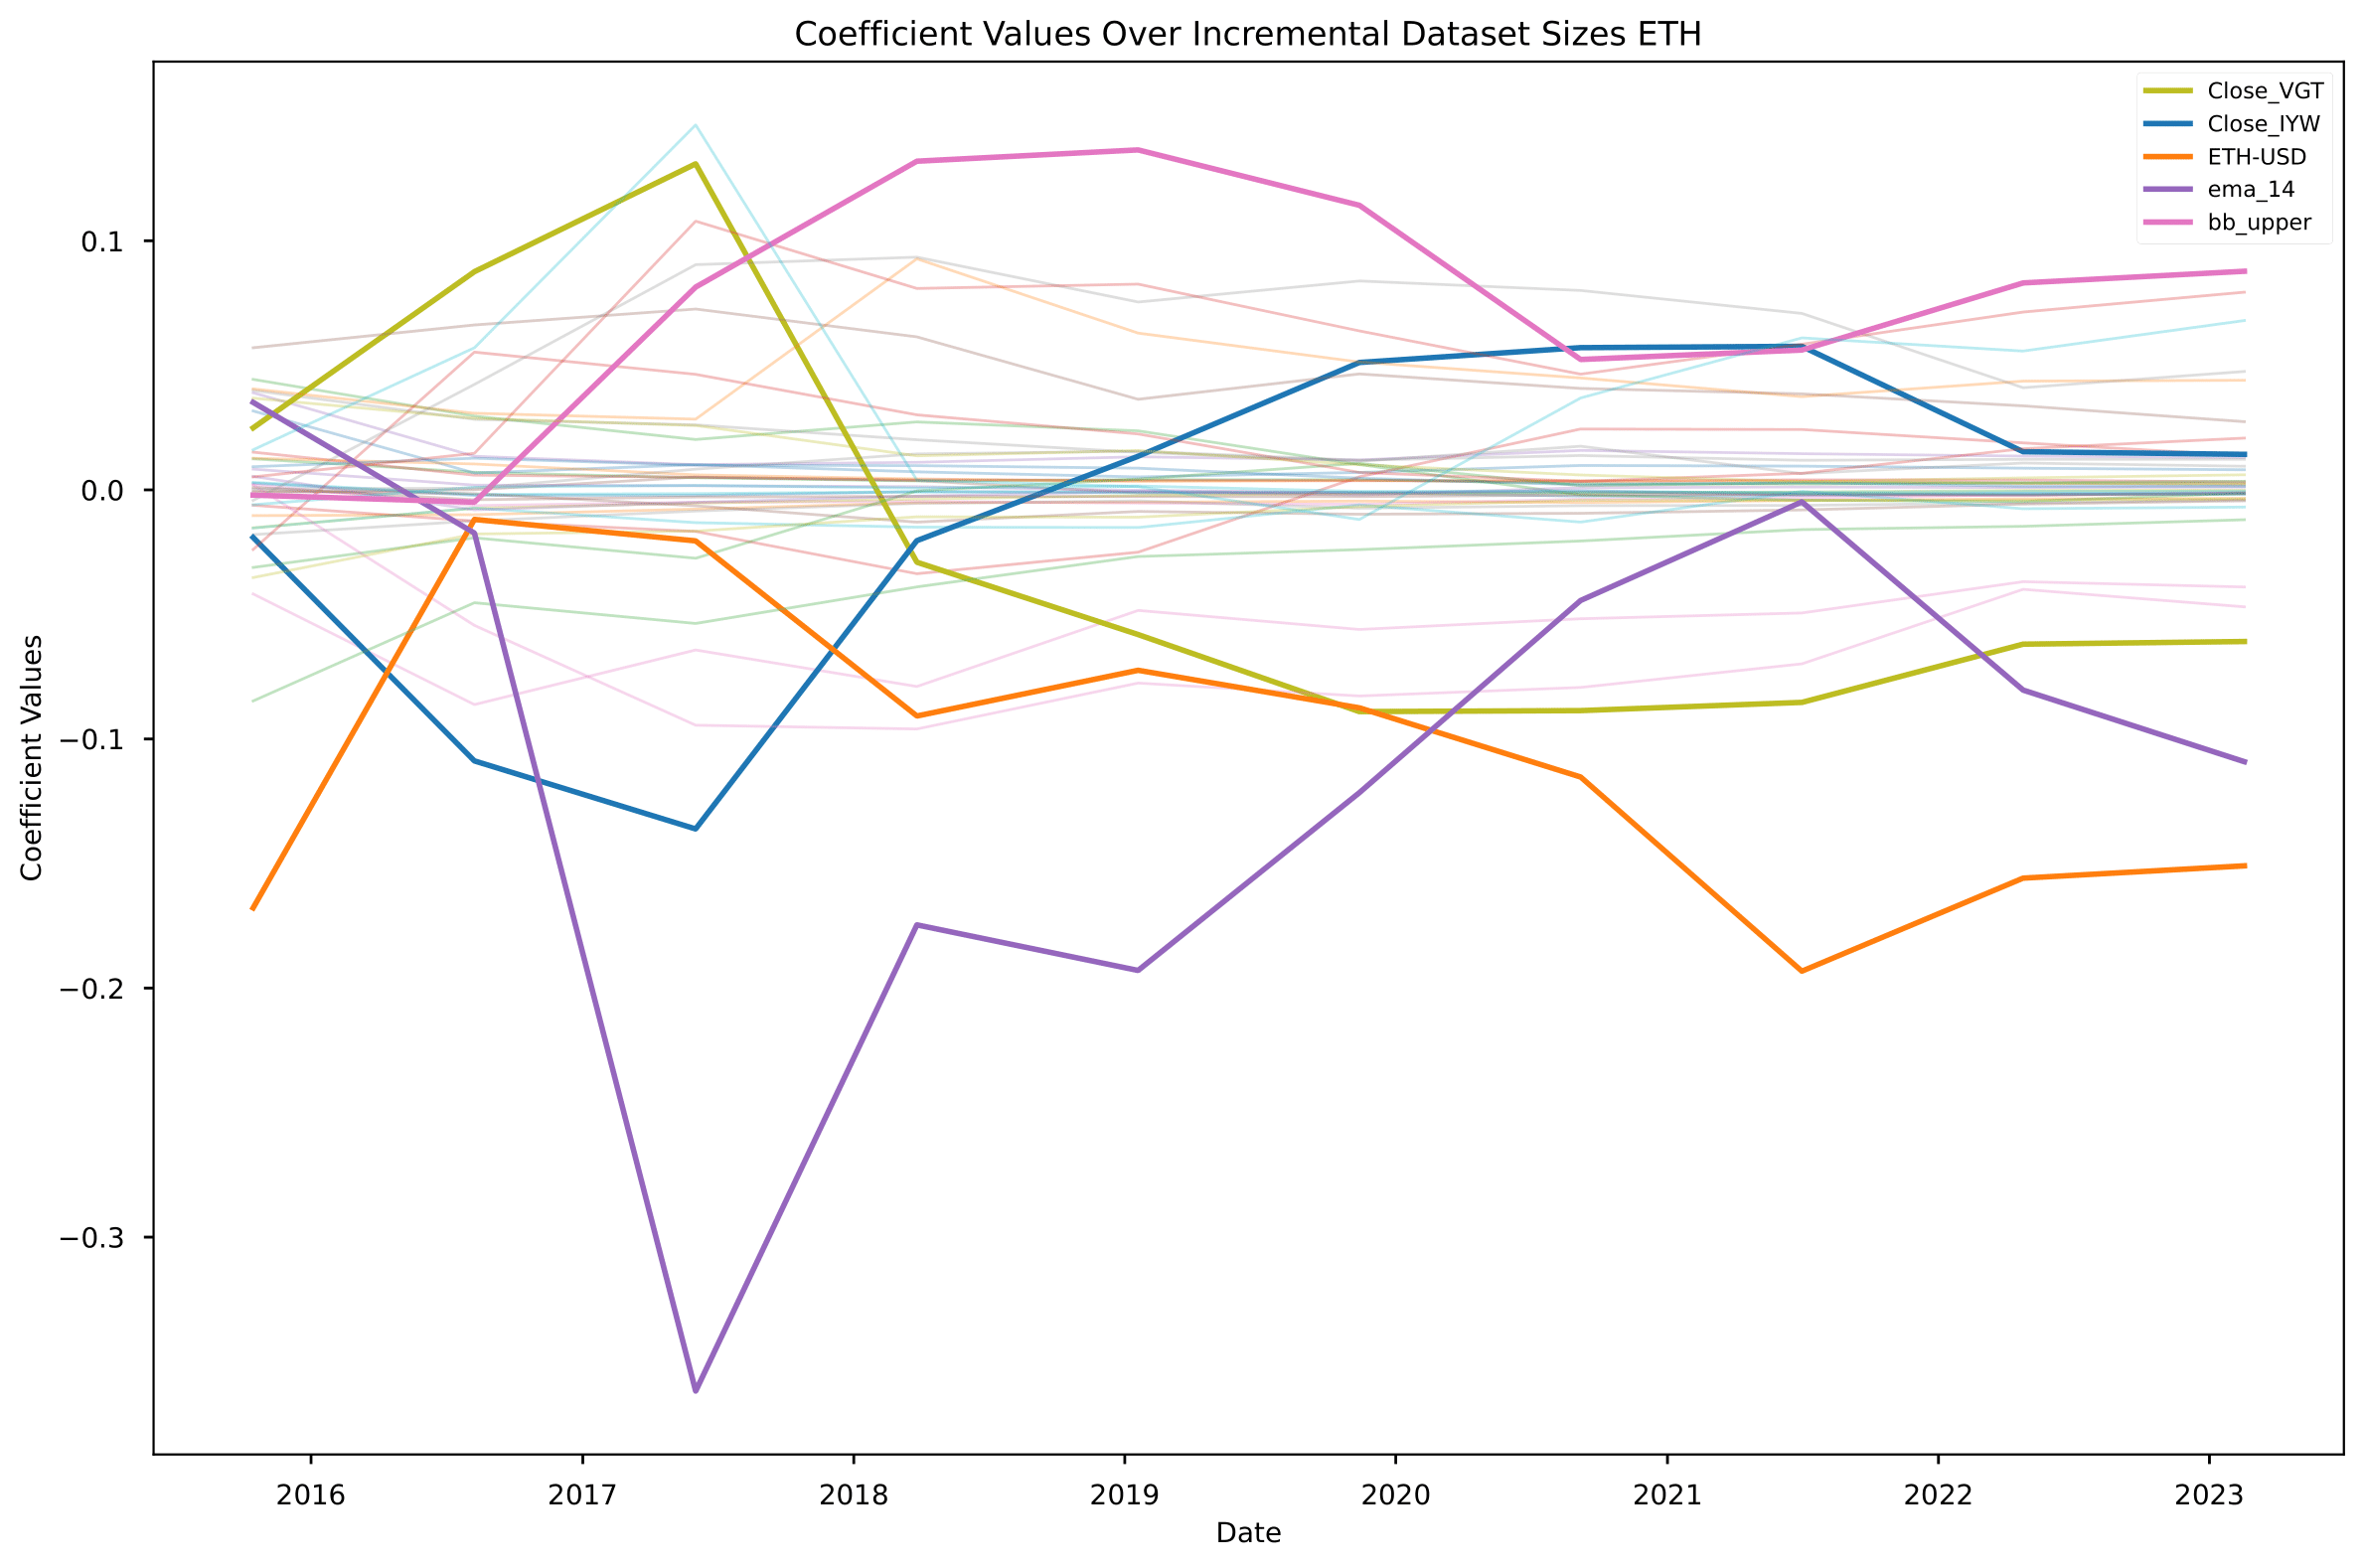
\includegraphics[width=1\textwidth]{Figures/coefficient_values_incremental_eth.png}
    \caption*{Source: Author}
    \label{fig:coefs_incremental_eth}
\end{figure}

\begin{figure}[!h]
    \centering
    \caption{Learned coefficients of the Ridge regression model
    with sliding window training on the ETH dataset. Five 
    coefficients with highest variance are highlighted.}
    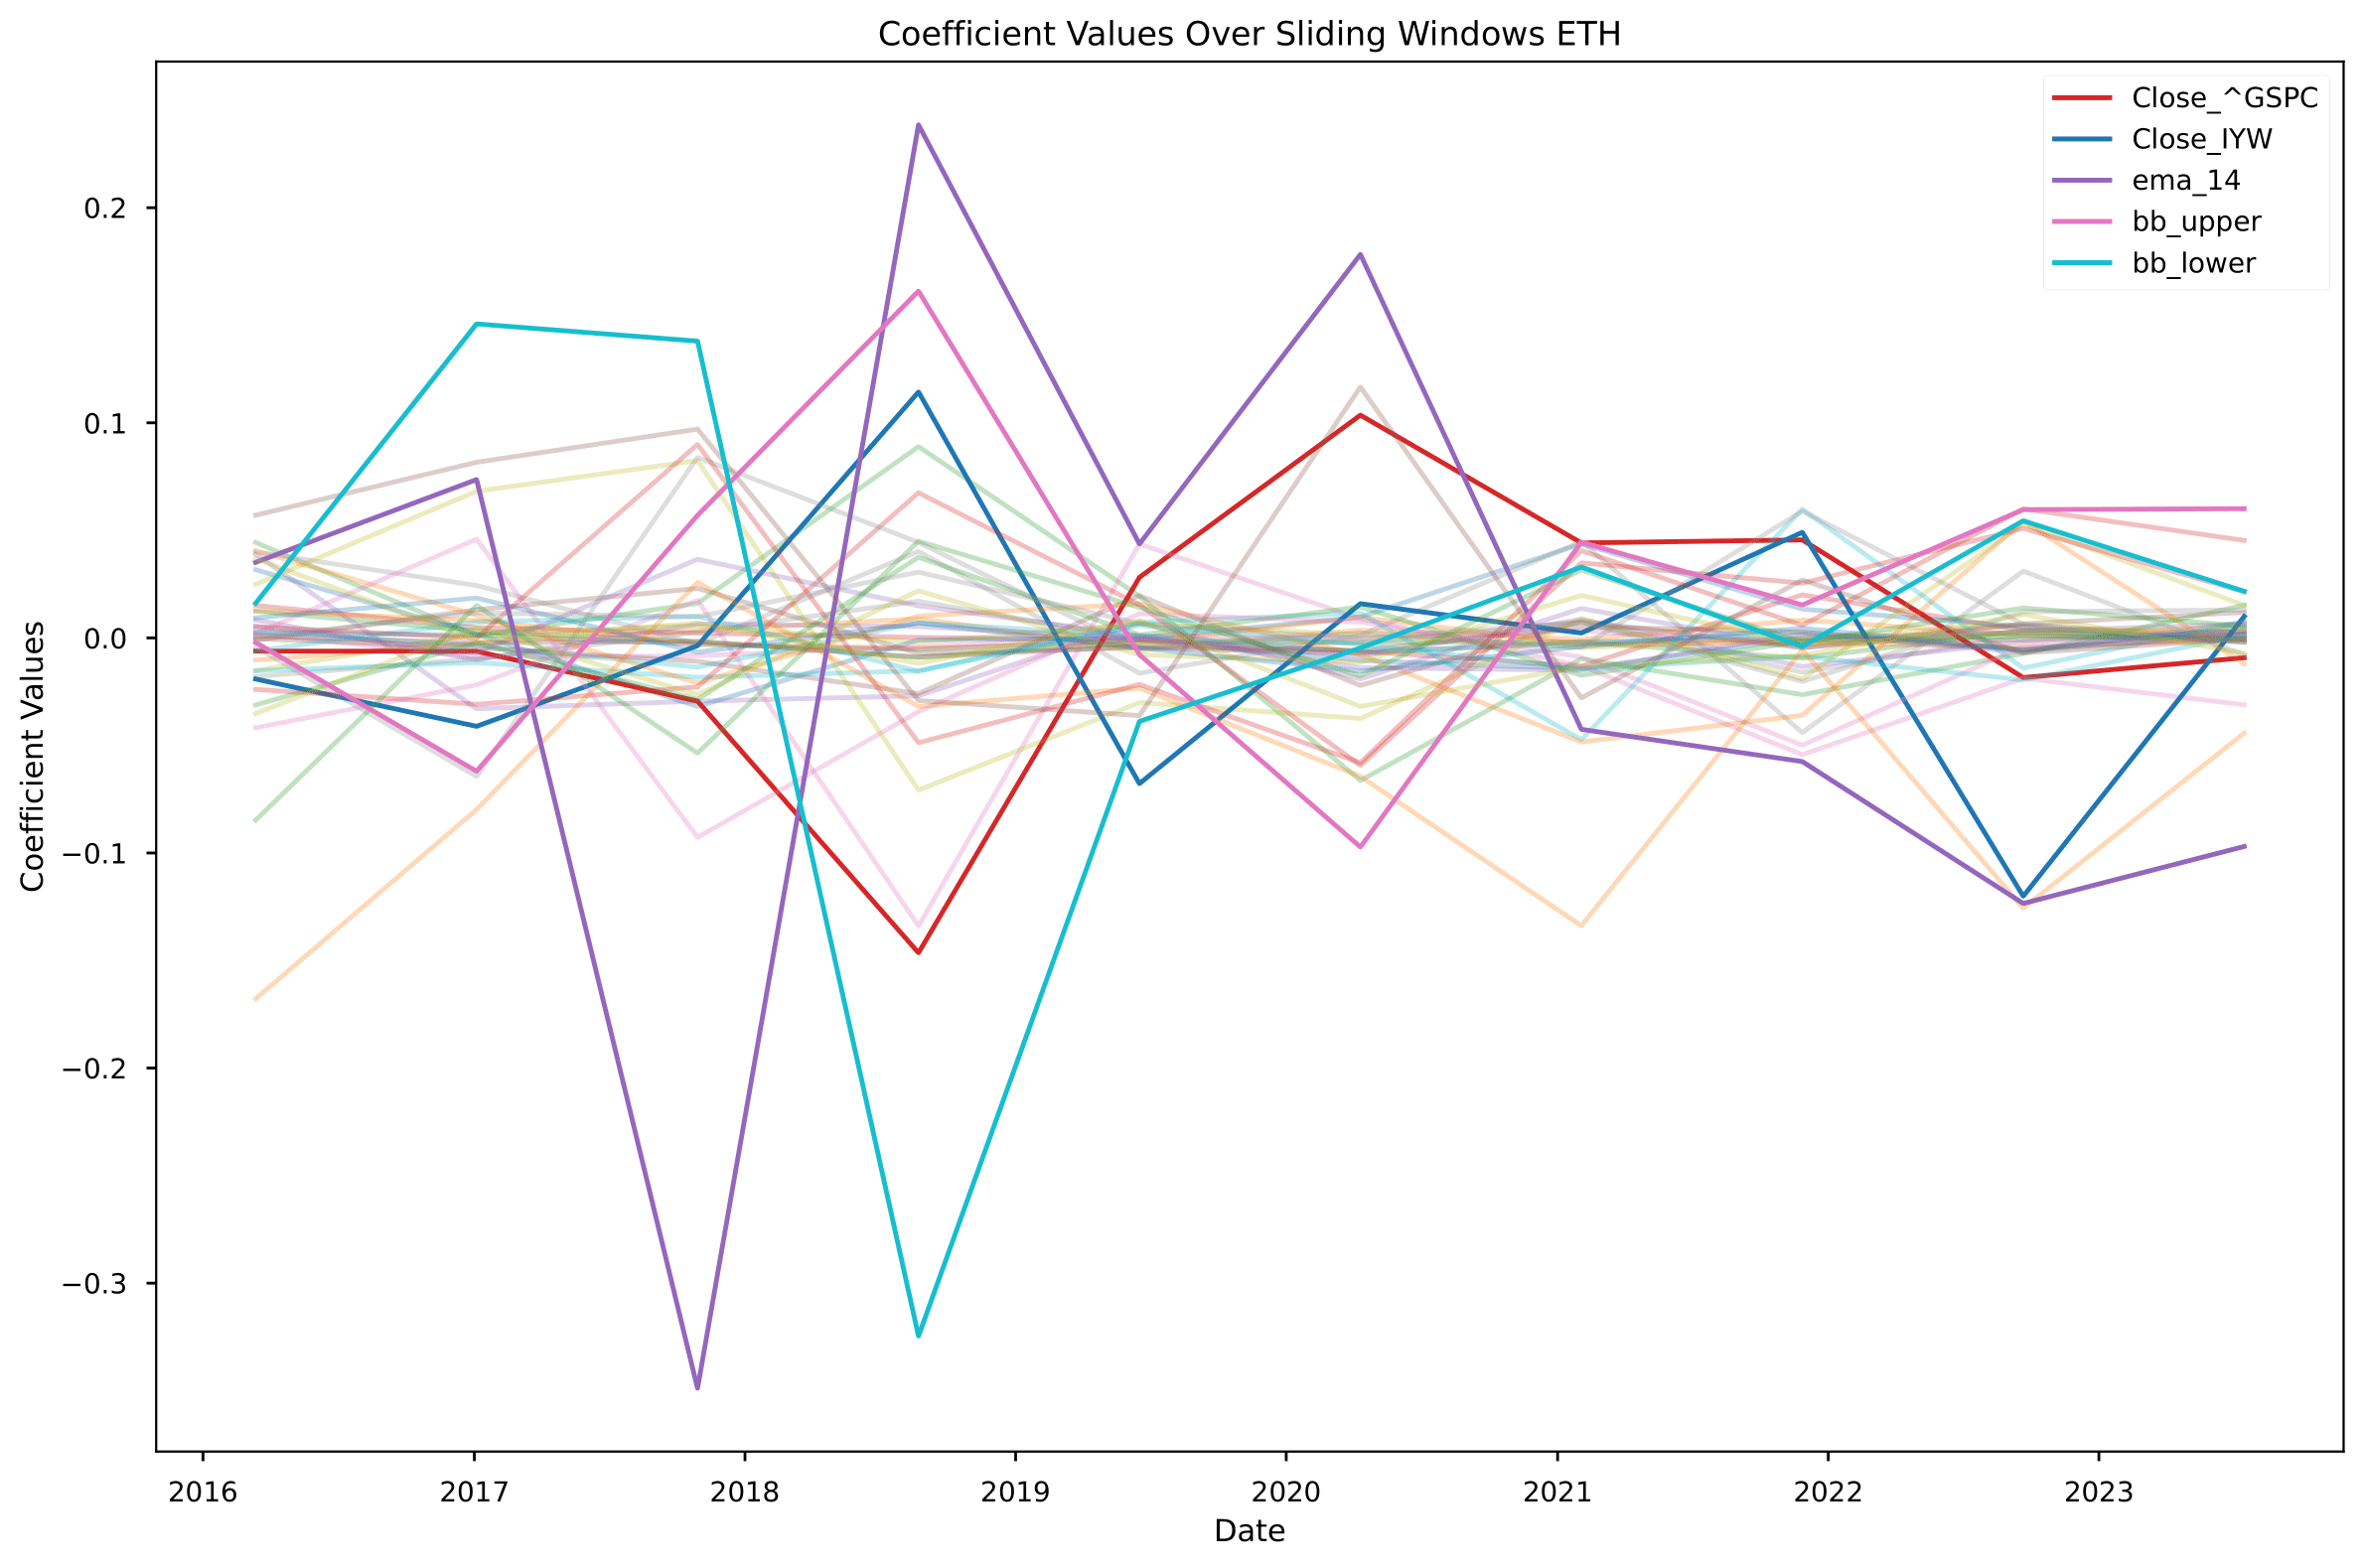
\includegraphics[width=1\textwidth]{Figures/coefficient_values_sliding_eth.png}
    \caption*{Source: Author}
    \label{fig:coefs_sliding_eth}
\end{figure}

\begin{figure}[!h]
    \centering
    \caption{Learned coefficients of the Ridge regression model
    with incremental training on the LTC dataset. Five 
    coefficients with highest variance are highlighted.}
    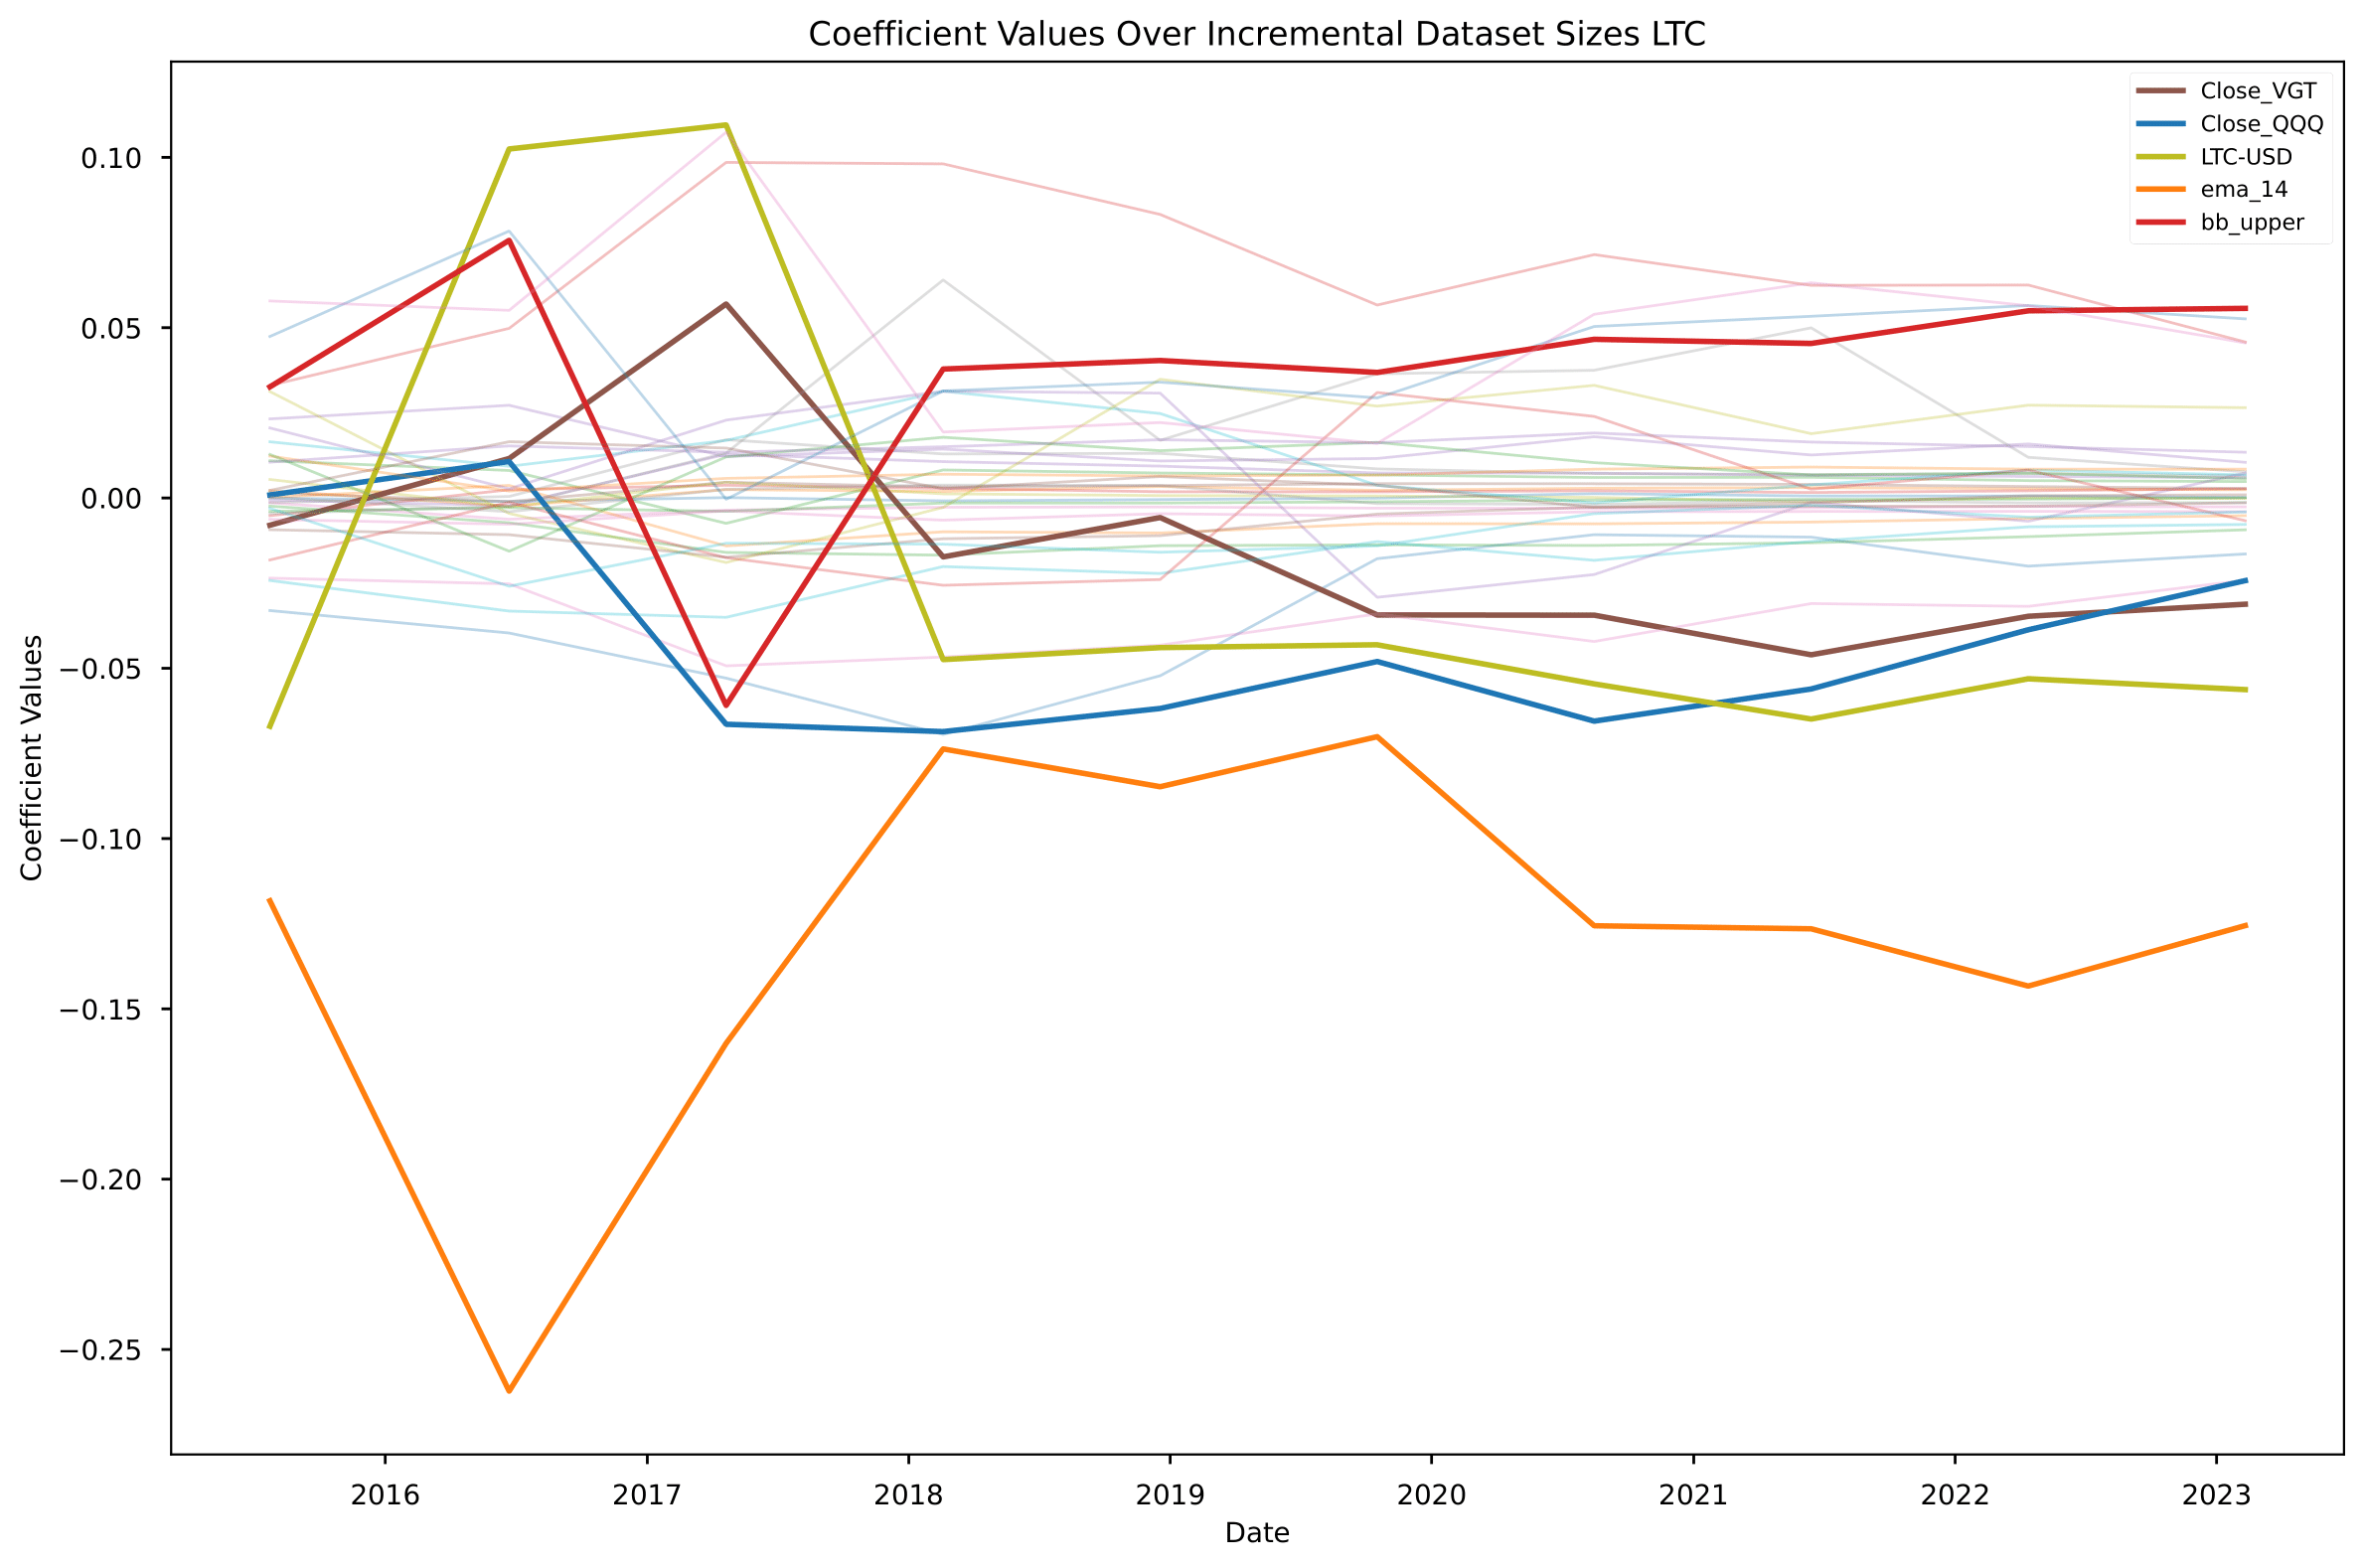
\includegraphics[width=1\textwidth]{Figures/coefficient_values_incremental_ltc.png}
    \caption*{Source: Author}
    \label{fig:coefs_incremental_ltc}
\end{figure}

\begin{figure}[!h]
    \centering
    \caption{Learned coefficients of the Ridge regression model
    with sliding window training on the LTC dataset. Five 
    coefficients with highest variance are highlighted.}
    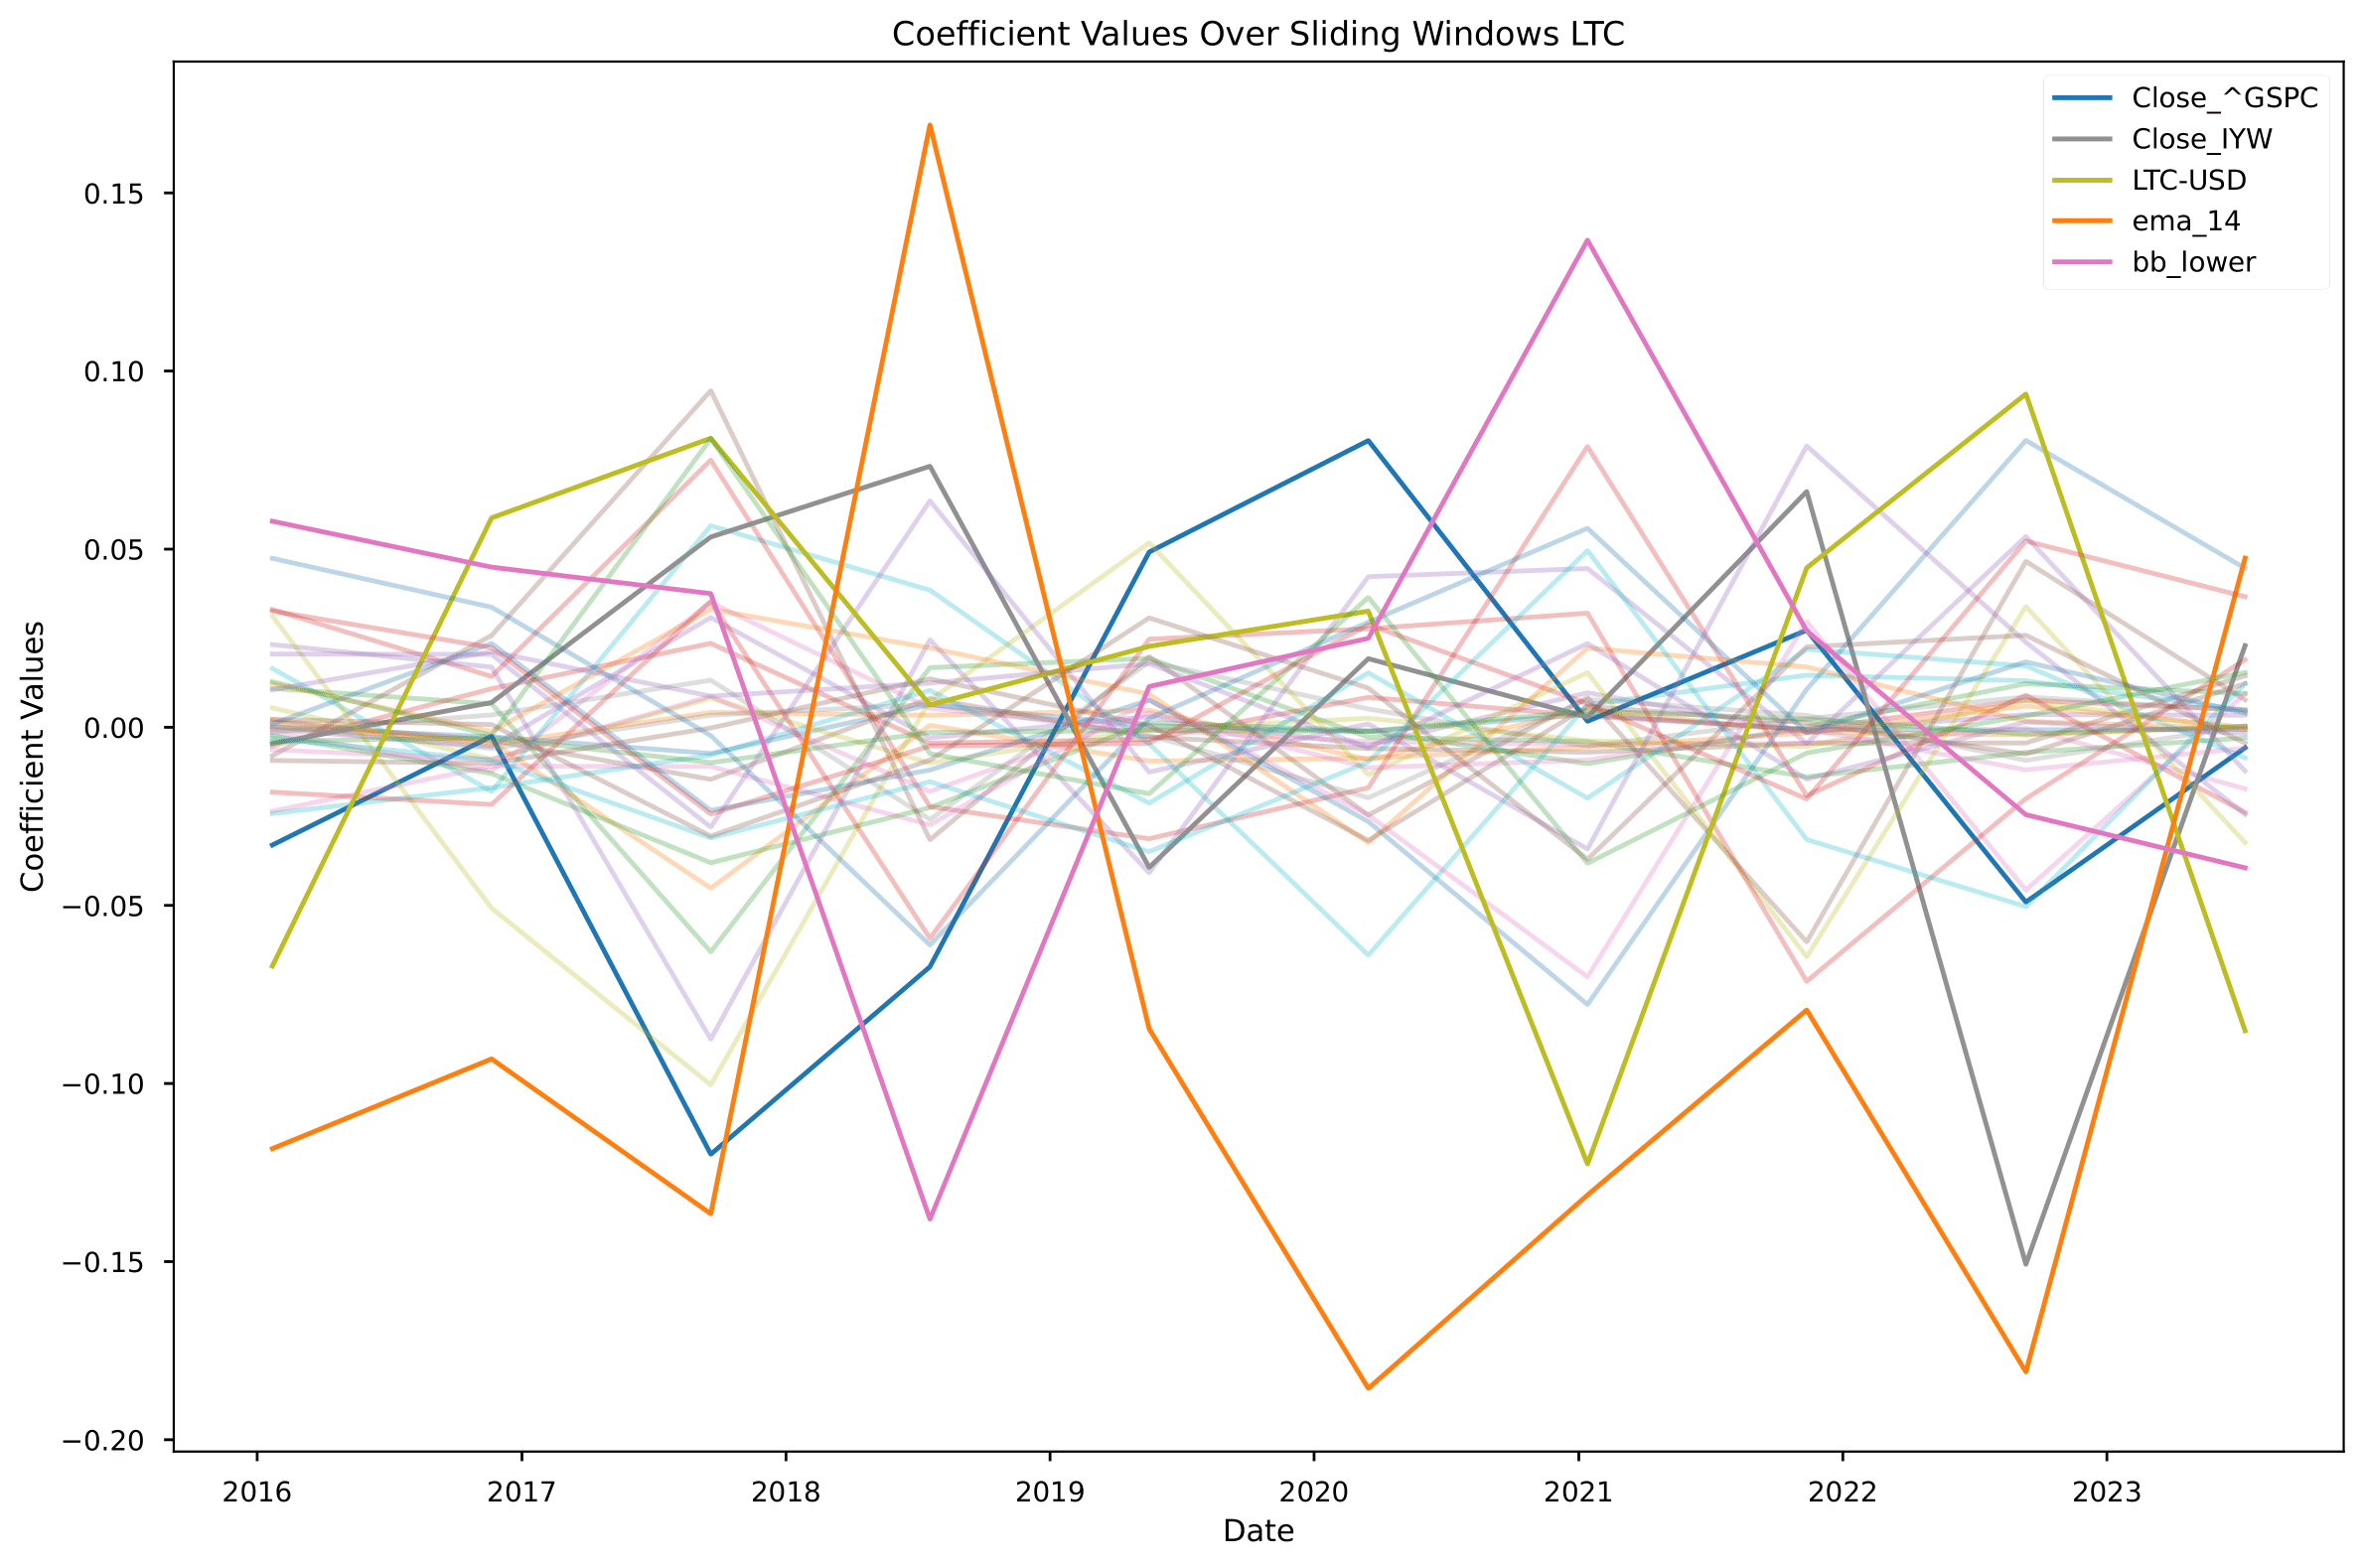
\includegraphics[width=1\textwidth]{Figures/coefficient_values_sliding_ltc.png}
    \caption*{Source: Author}
    \label{fig:coefs_sliding_ltc}
\end{figure}



